\documentclass[usepdftitle=false]{beamer}

\usepackage[T1]{fontenc}

\usepackage[utf8x]{inputenc}
\usepackage{default}
\usepackage{lmodern}
\usepackage{booktabs}

\usepackage{ragged2e} % Kommando\justifying ermöglicht  Blocksatz in Präsentationen

\mode<presentation>
 {\usecolortheme{seahorse,rose}
 \useinnertheme[shadow]{rounded}
%  \useoutertheme[hideothersubsections,right,width=4em,frame number]{sidebar}
%  \useoutertheme{infolines}
%\useoutertheme{split}
\useoutertheme[subsection=false,footline=authortitle]{miniframes}
\setbeamercovered{transparent}
}

%seitenzahl in linker ecke
\addtobeamertemplate{navigation symbols}{{\usebeamercolor{section
in toc}\footnotesize
\insertframenumber/\inserttotalframenumber}\hspace{48em}}{}
\usepackage{setspace} %mit spacing-Umgebung Zeilenabstand regeln



%%Sprachunterstuetzung
%Englische Silbentrennung, etc.
\usepackage[spanish]{babel}
%Mehrsprachige Literaturliste
\usepackage{babelbib}
%%Graphiken und Farbe
%Graphiken
\usepackage{graphicx} 
%von beamer.cls geladen
%Farbe
\usepackage{color,pgf}
%von beamer.cls geladen
%PDF-Seiten einbinden
\usepackage{pdfpages}
\usepackage{subscript}
\newcommand{\sub}[1]{\textsubscript{#1}}
\newcommand{\Sup}[1]{\textsuperscript{#1}}
\newcommand{\COO}{CO\textsubscript{2}}
\newcommand{\masl}{m~a.s.l.}
\newcommand{\gc}{$^{\circ}$C}
\newcommand{\tilt}{$\sim$}
\newcommand{\blue}[1]{{\color{blue!50!black}#1}}
\newcommand{\Blue}[1]{{\color{blue!50!black}\textbf{#1}}}
\newcommand{\eg}{e.\,g.}
\newcommand{\Eg}{E.\,g.}

% new environment for slides with changes margins
\newenvironment{changemargin}[2]{%
\begin{list}{}{%
\setlength{\topsep}{0pt}%
\setlength{\leftmargin}{#1}%
\setlength{\rightmargin}{#2}%
\setlength{\listparindent}{\parindent}%
\setlength{\itemindent}{\parindent}%
\setlength{\parsep}{\parskip}%
}%
\item[]}{\end{list}}





\hypersetup{
pdfauthor={Roman Link},
pdftitle={El método de Bench Dehydration},
}

%Titelseite
\title{El método de Bench Dehydration}
\subtitle{\normalfont Curso de laboratorio \textit{Mediciones de hidráulica de plantas con el XylEm Plus y la bomba de Scholander}}
\author[R. Link]{Roman Link}
\date{27 de noviembre de 2017}
\institute[University of Göttingen]{
Department of Plant Ecology and Ecosystem Research\\ Georg August University of Göttingen}
%\titlegraphic{ \vspace*{2em}
%
\includegraphics[width=0.7\textwidth]{logouni.png}}%oder was sch\"oneres

\logo{
\includegraphics[width=20em]{logounisolow.png}}

\usepackage{amsmath,amsfonts,amssymb,pgf}
 \usepackage { eulervm }

%\usepackage[round]{natbib}
%\def\newblock{} % hilft gegen absurde fehler mit natbib

\newcommand{\rar}{$\rightarrow$}
\newcommand{\lar}{$\leftarrow$}
\newcommand{\Rar}{$\Rightarrow$}
\newcommand{\Lar}{$\Leftarrow$}
\newcommand{\quelle}[1]{\baselineskip8pt{\tiny \color{gray} #1}}

\newcommand{\tw}{\textwidth}
\newcommand{\ddx}[2]{\frac{\mathrm{d}}{\mathrm{d}#2}#1 }
\newcommand{\ddxx}[2]{\frac{\mathrm{d^2}}{\mathrm{d}#2^2}#1}



\newcommand{\code}[1]{{\footnotesize \color{blue}
\texttt{#1}}\normalsize\color{black}}


% \input{cc_beamer}
\setbeamerfont{section in toc}{size=\normalsize,series=\bfseries}
\setbeamerfont{title}{series=\bfseries}
\setbeamerfont{frametitle}{size=\Large,series=\bfseries}

\begin{document}


%%%%%%%%%%%%%%%%%		Title Page			%%%%%%%%%%%%%%%%%%%%%%
\begin{frame}
\titlepage
\end{frame}

%%%%%%%%%%%%%%%%%%%%%%%%%%%%%%%%%%%%%%%%%%%%%%%%%%%%%%%%%%%%%%%%%%%%%%%%
\section{Protocolo de medición}
%%%%%%%%%%%%%%%%%%%%%%%%%%%%%%%%%%%%%%%%%%%%%%%%%%%%%%%%%%%%%%%%%%%%%%%%
% copiar de Prometheus Wiki
\begin{frame}	
	\centering
	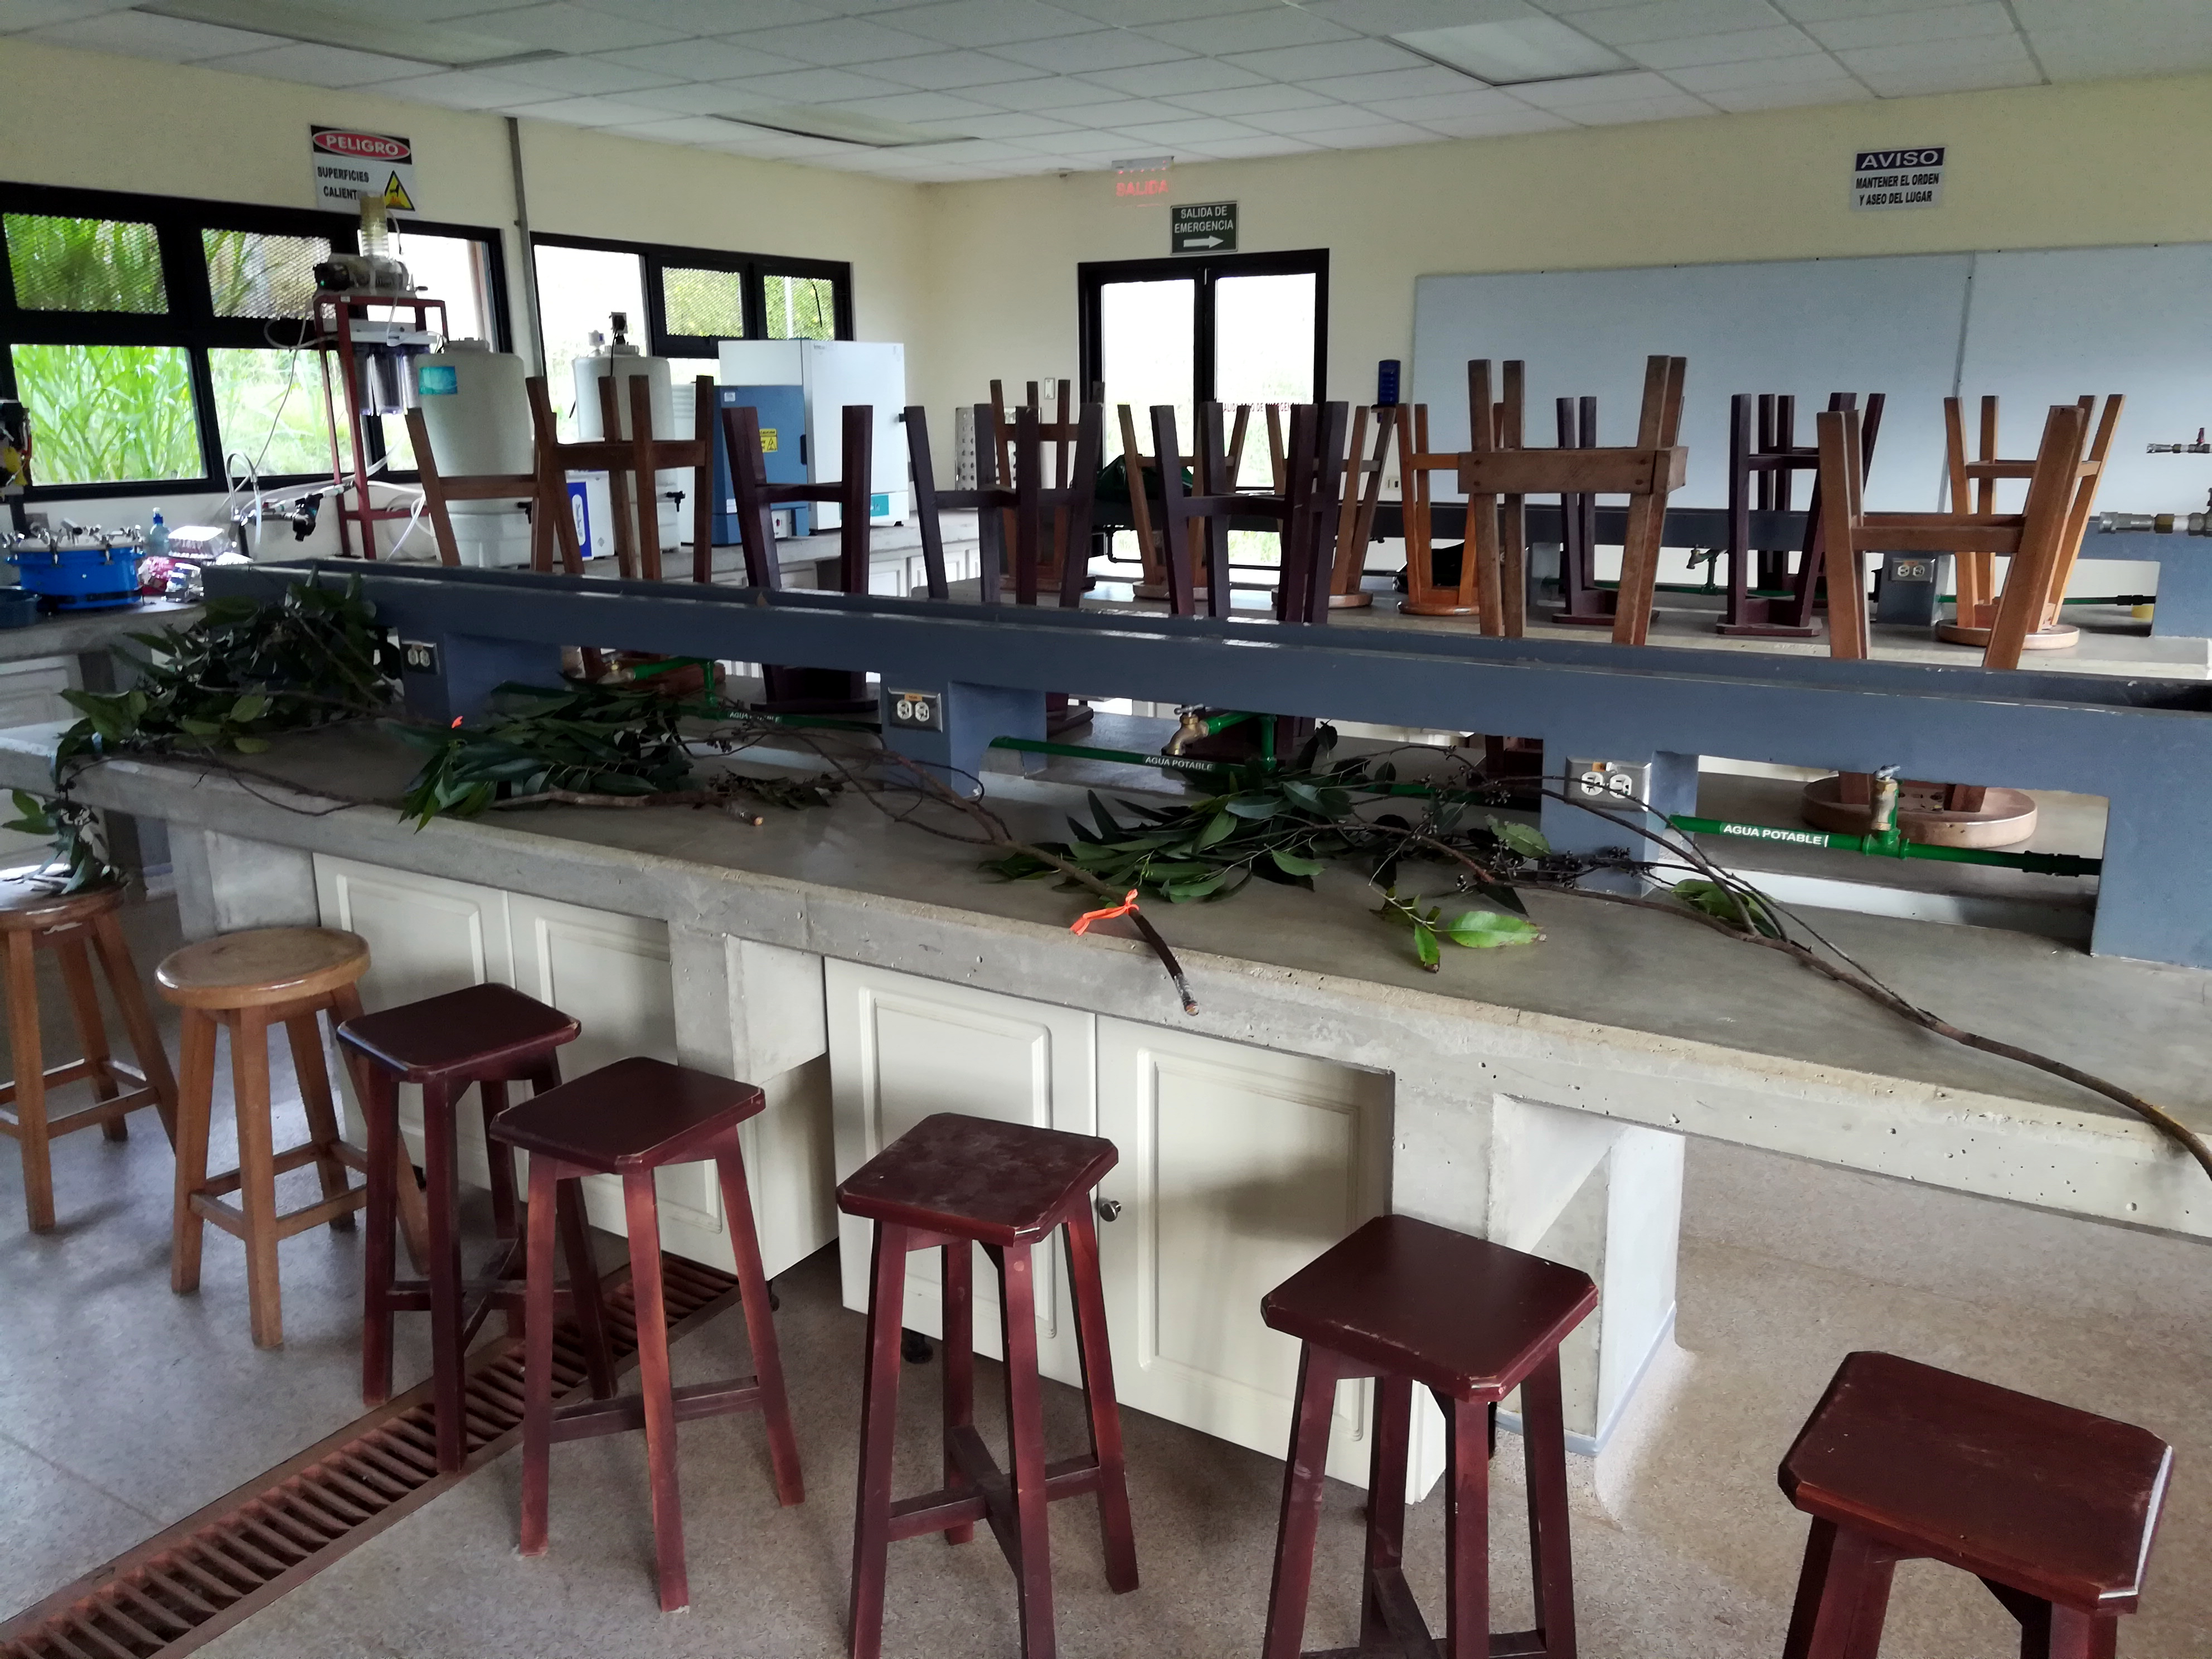
\includegraphics[width = 0.7\tw]{pictures/bench_drying.jpg}
	\begin{block}{\textbf{Bench dehydration}}
	    Deshidratación en la mesa de laboratorio (\textit{laboratory bench})
	\end{block}
\end{frame}

\begin{frame}
\frametitle{Toma de muestras}
\begin{minipage}{0.48\tw}
\centering
\only<1>{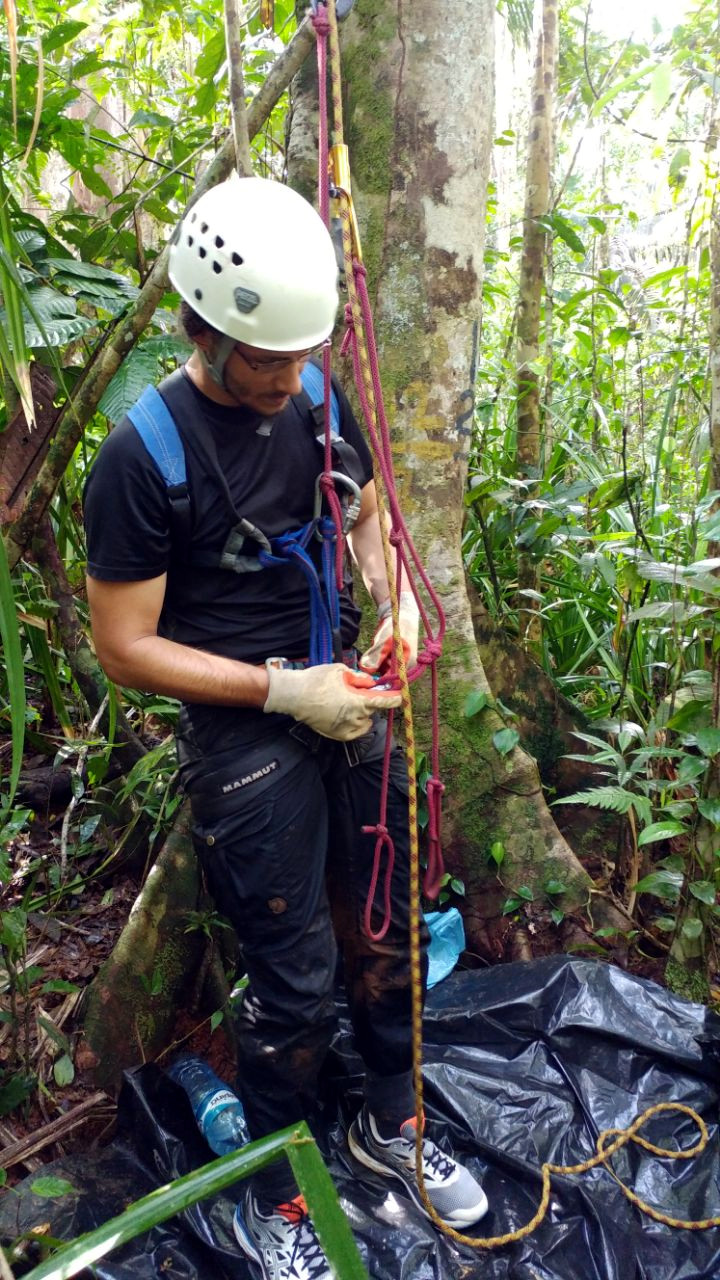
\includegraphics[height = 0.9\textheight]{pictures/field4.jpg}}
\only<2>{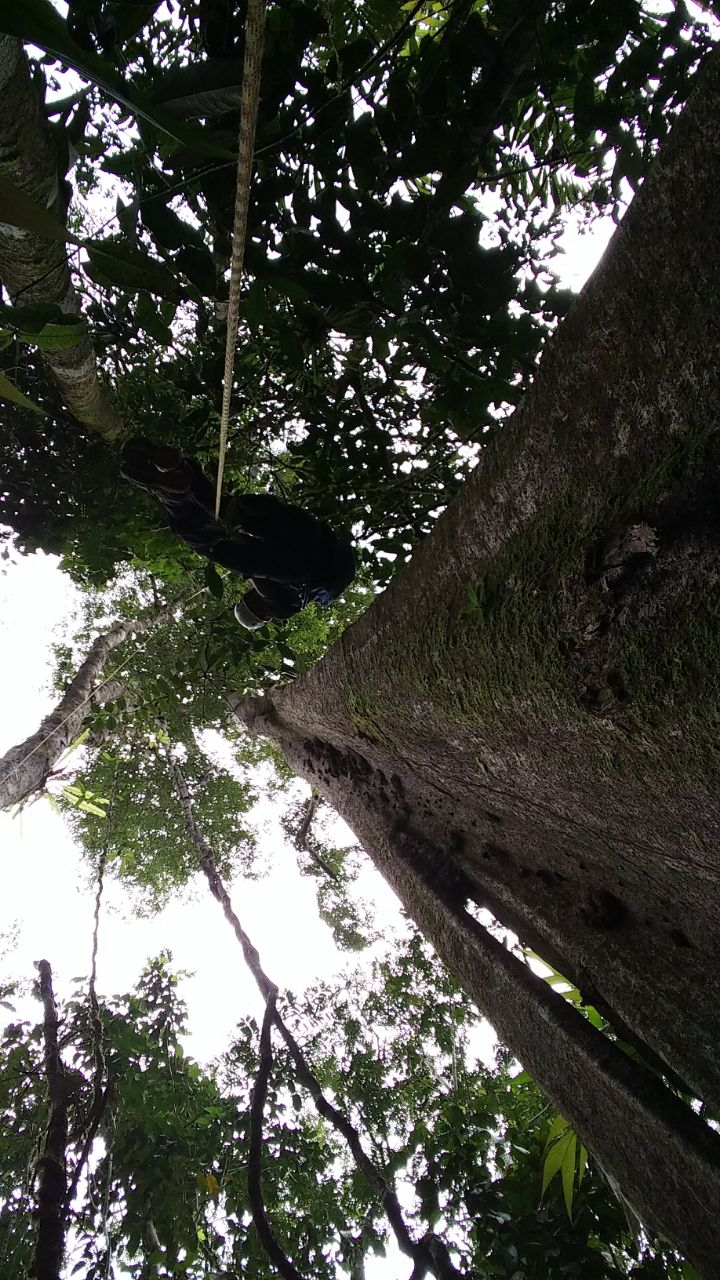
\includegraphics[height = 0.9\textheight]{pictures/field5.jpg}}
\only<3>{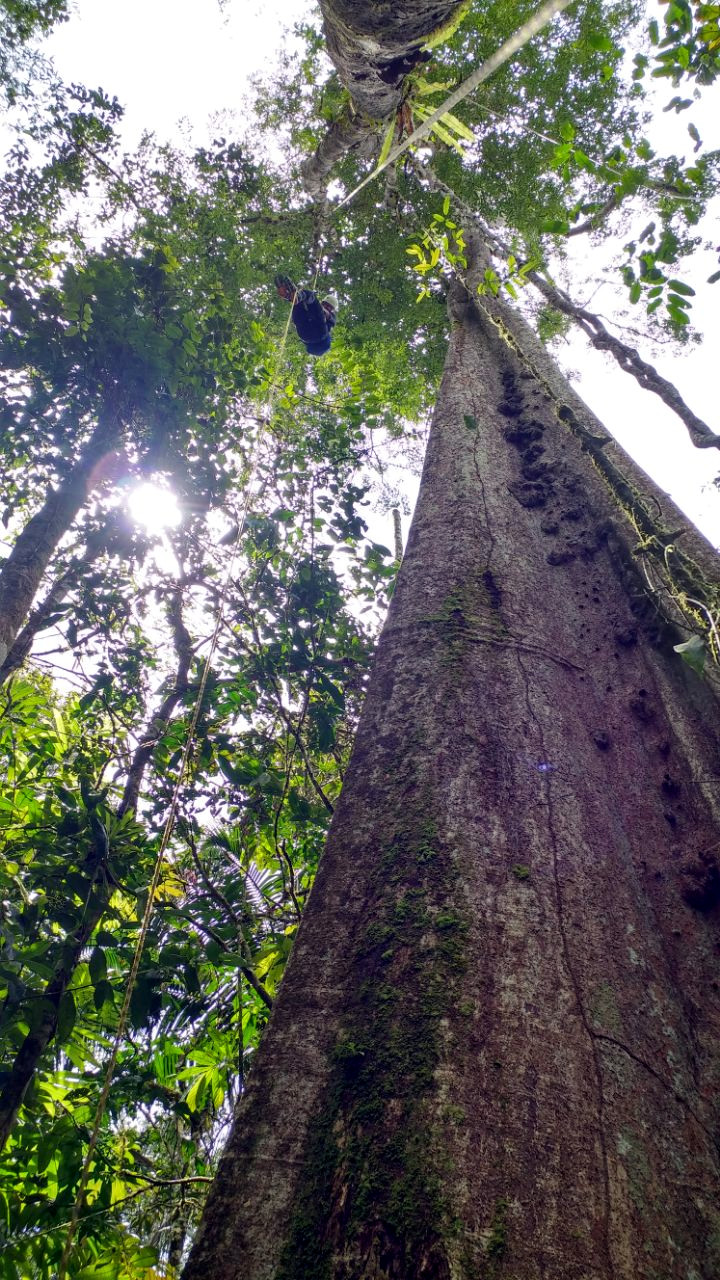
\includegraphics[height = 0.9\textheight]{pictures/field3.jpg}}
\only<4>{\includegraphics[width = \tw]{pictures/field1.jpg}}
\end{minipage}
\begin{minipage}{0.5\tw}
\begin{itemize}[<+-| alert@+>]
	\item Idealmente tomar muestras de la parte de la copa que tiene exposición directa a la luz solar (hay que escalar...)
	\item Después de cortar, inmediatamente ponerlas en un cubo de agua y cortar parte basípeta bajo agua 
	\item Tiempo ideal para la toma de muestras: Justo antes del amanecer
    \item Longitud recomendada: más que 1.5x la longitud máxima de vasos    
\end{itemize}	
\end{minipage}
\end{frame}
	
	\begin{frame}
\centering{\includegraphics[height = 0.9\textheight]{pictures/field2.jpg}}	
	\end{frame}



\begin{frame}
	\frametitle{Rehidratación}
\begin{minipage}{0.38\tw}
	\centering
	\only<1>{
	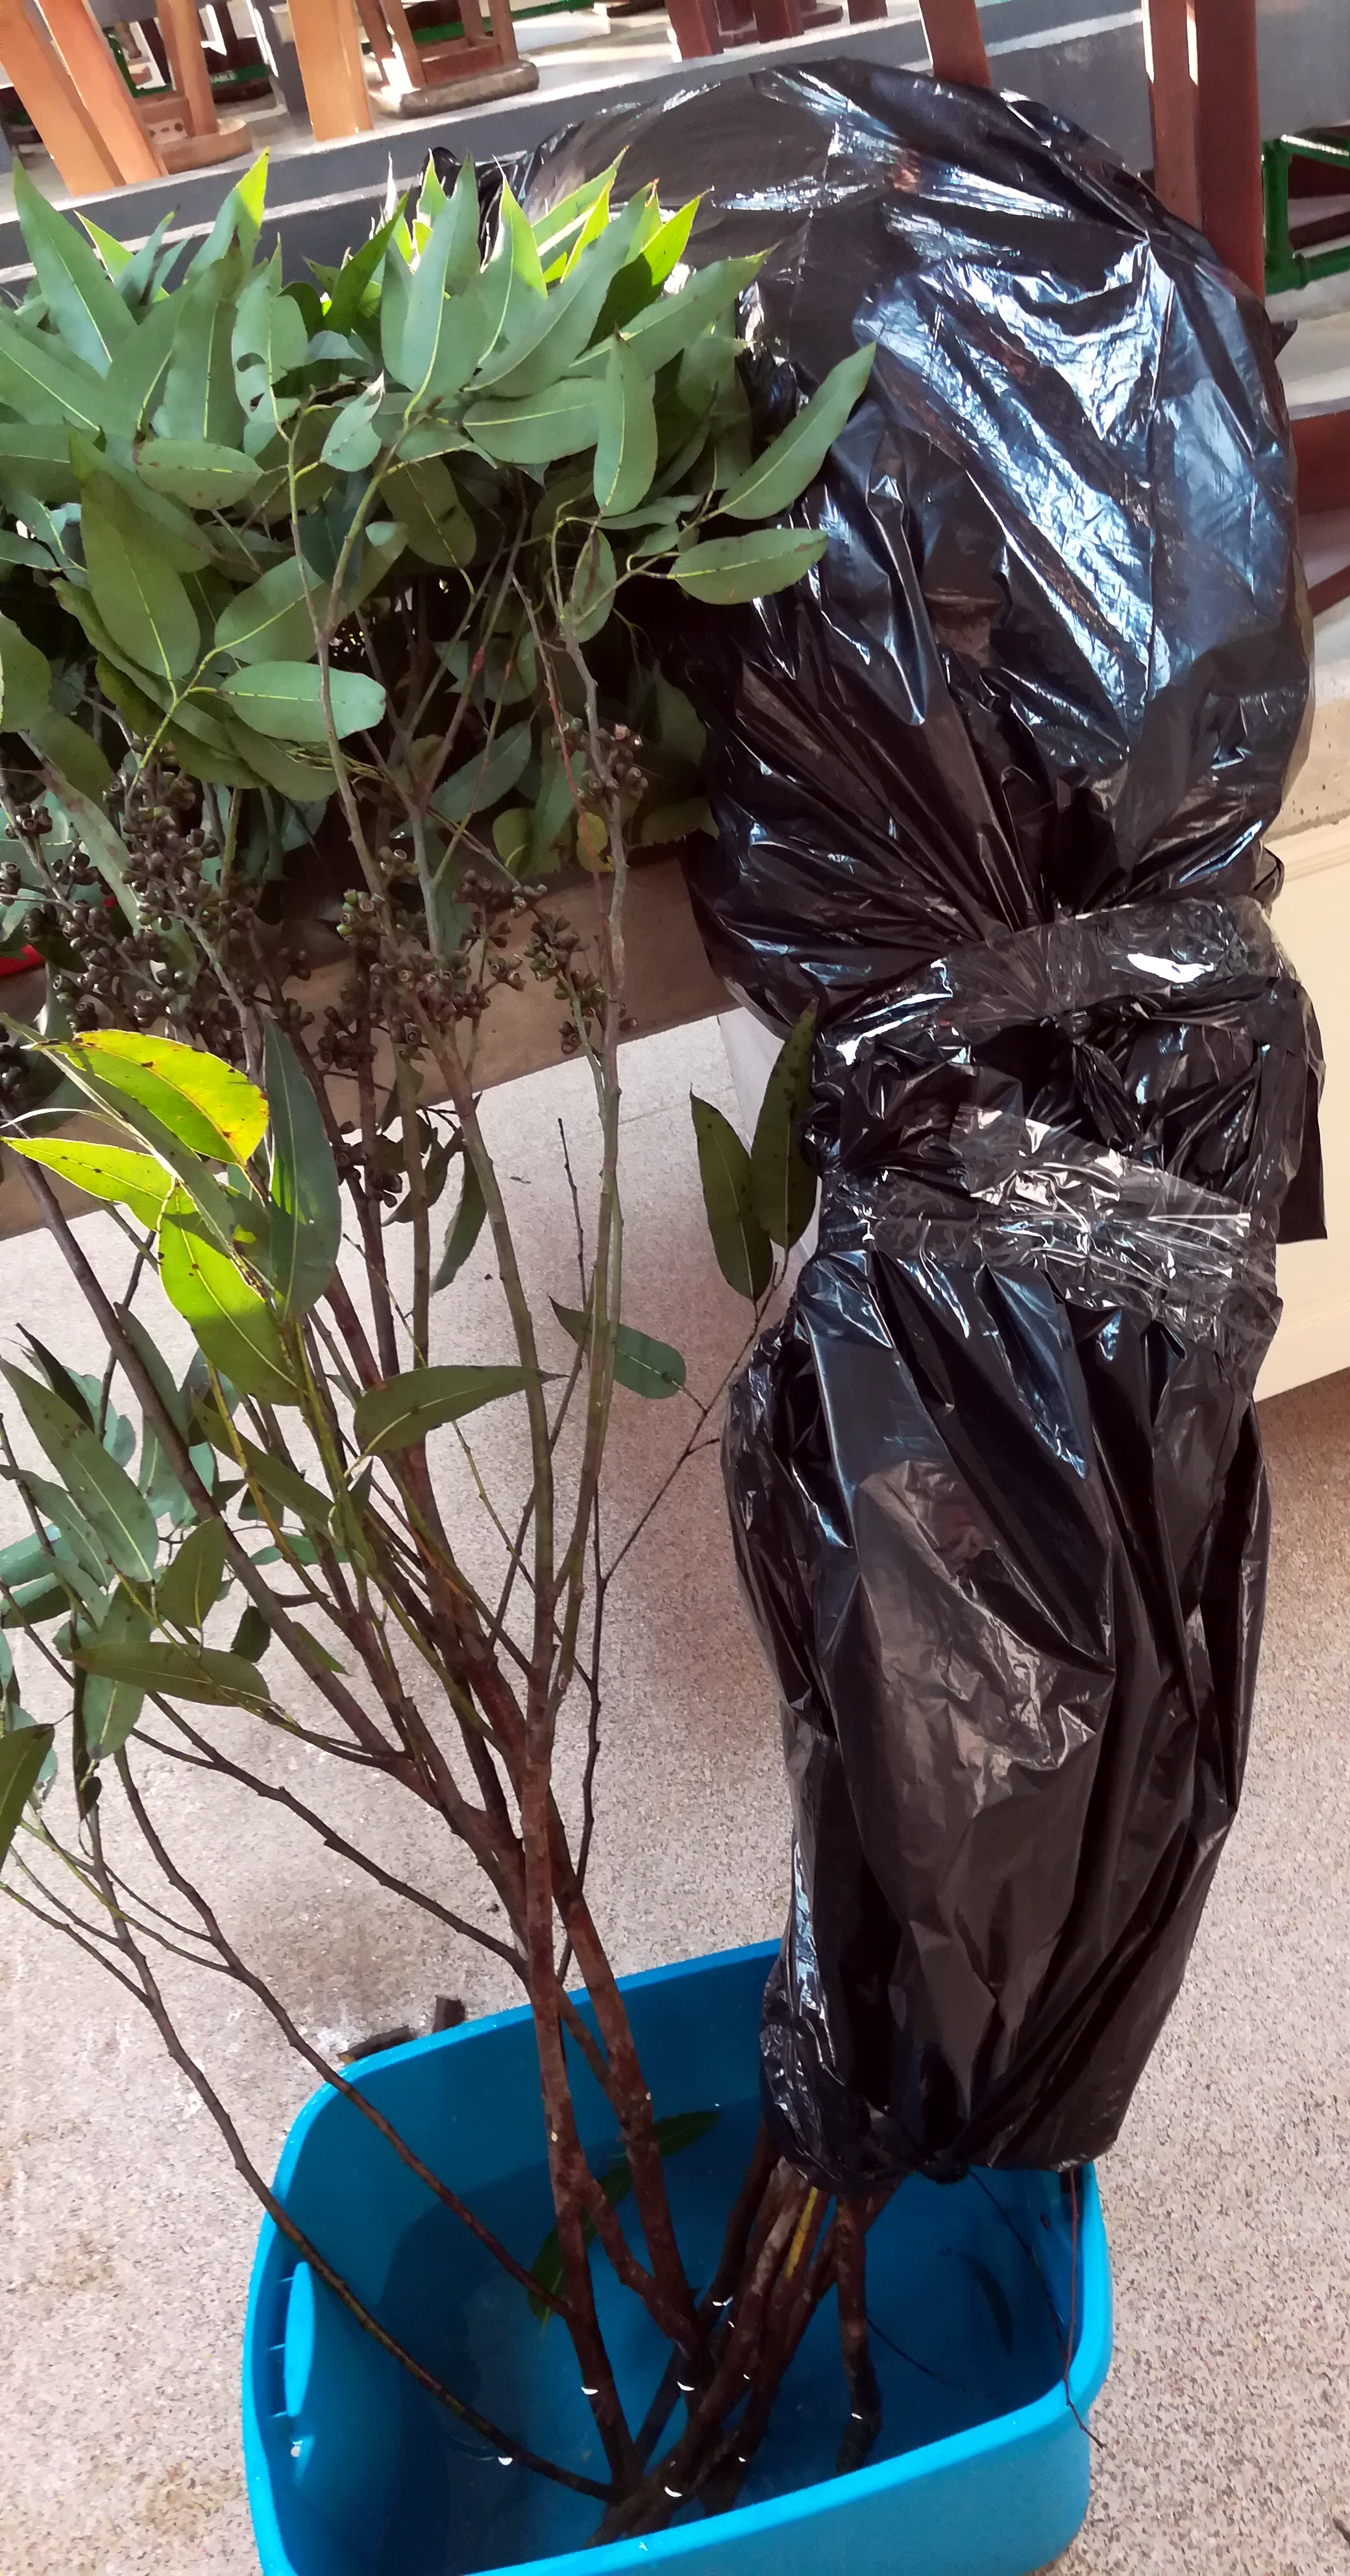
\includegraphics[height = 0.85\textheight]{pictures/bagging.jpg}}
	\only<2>{
	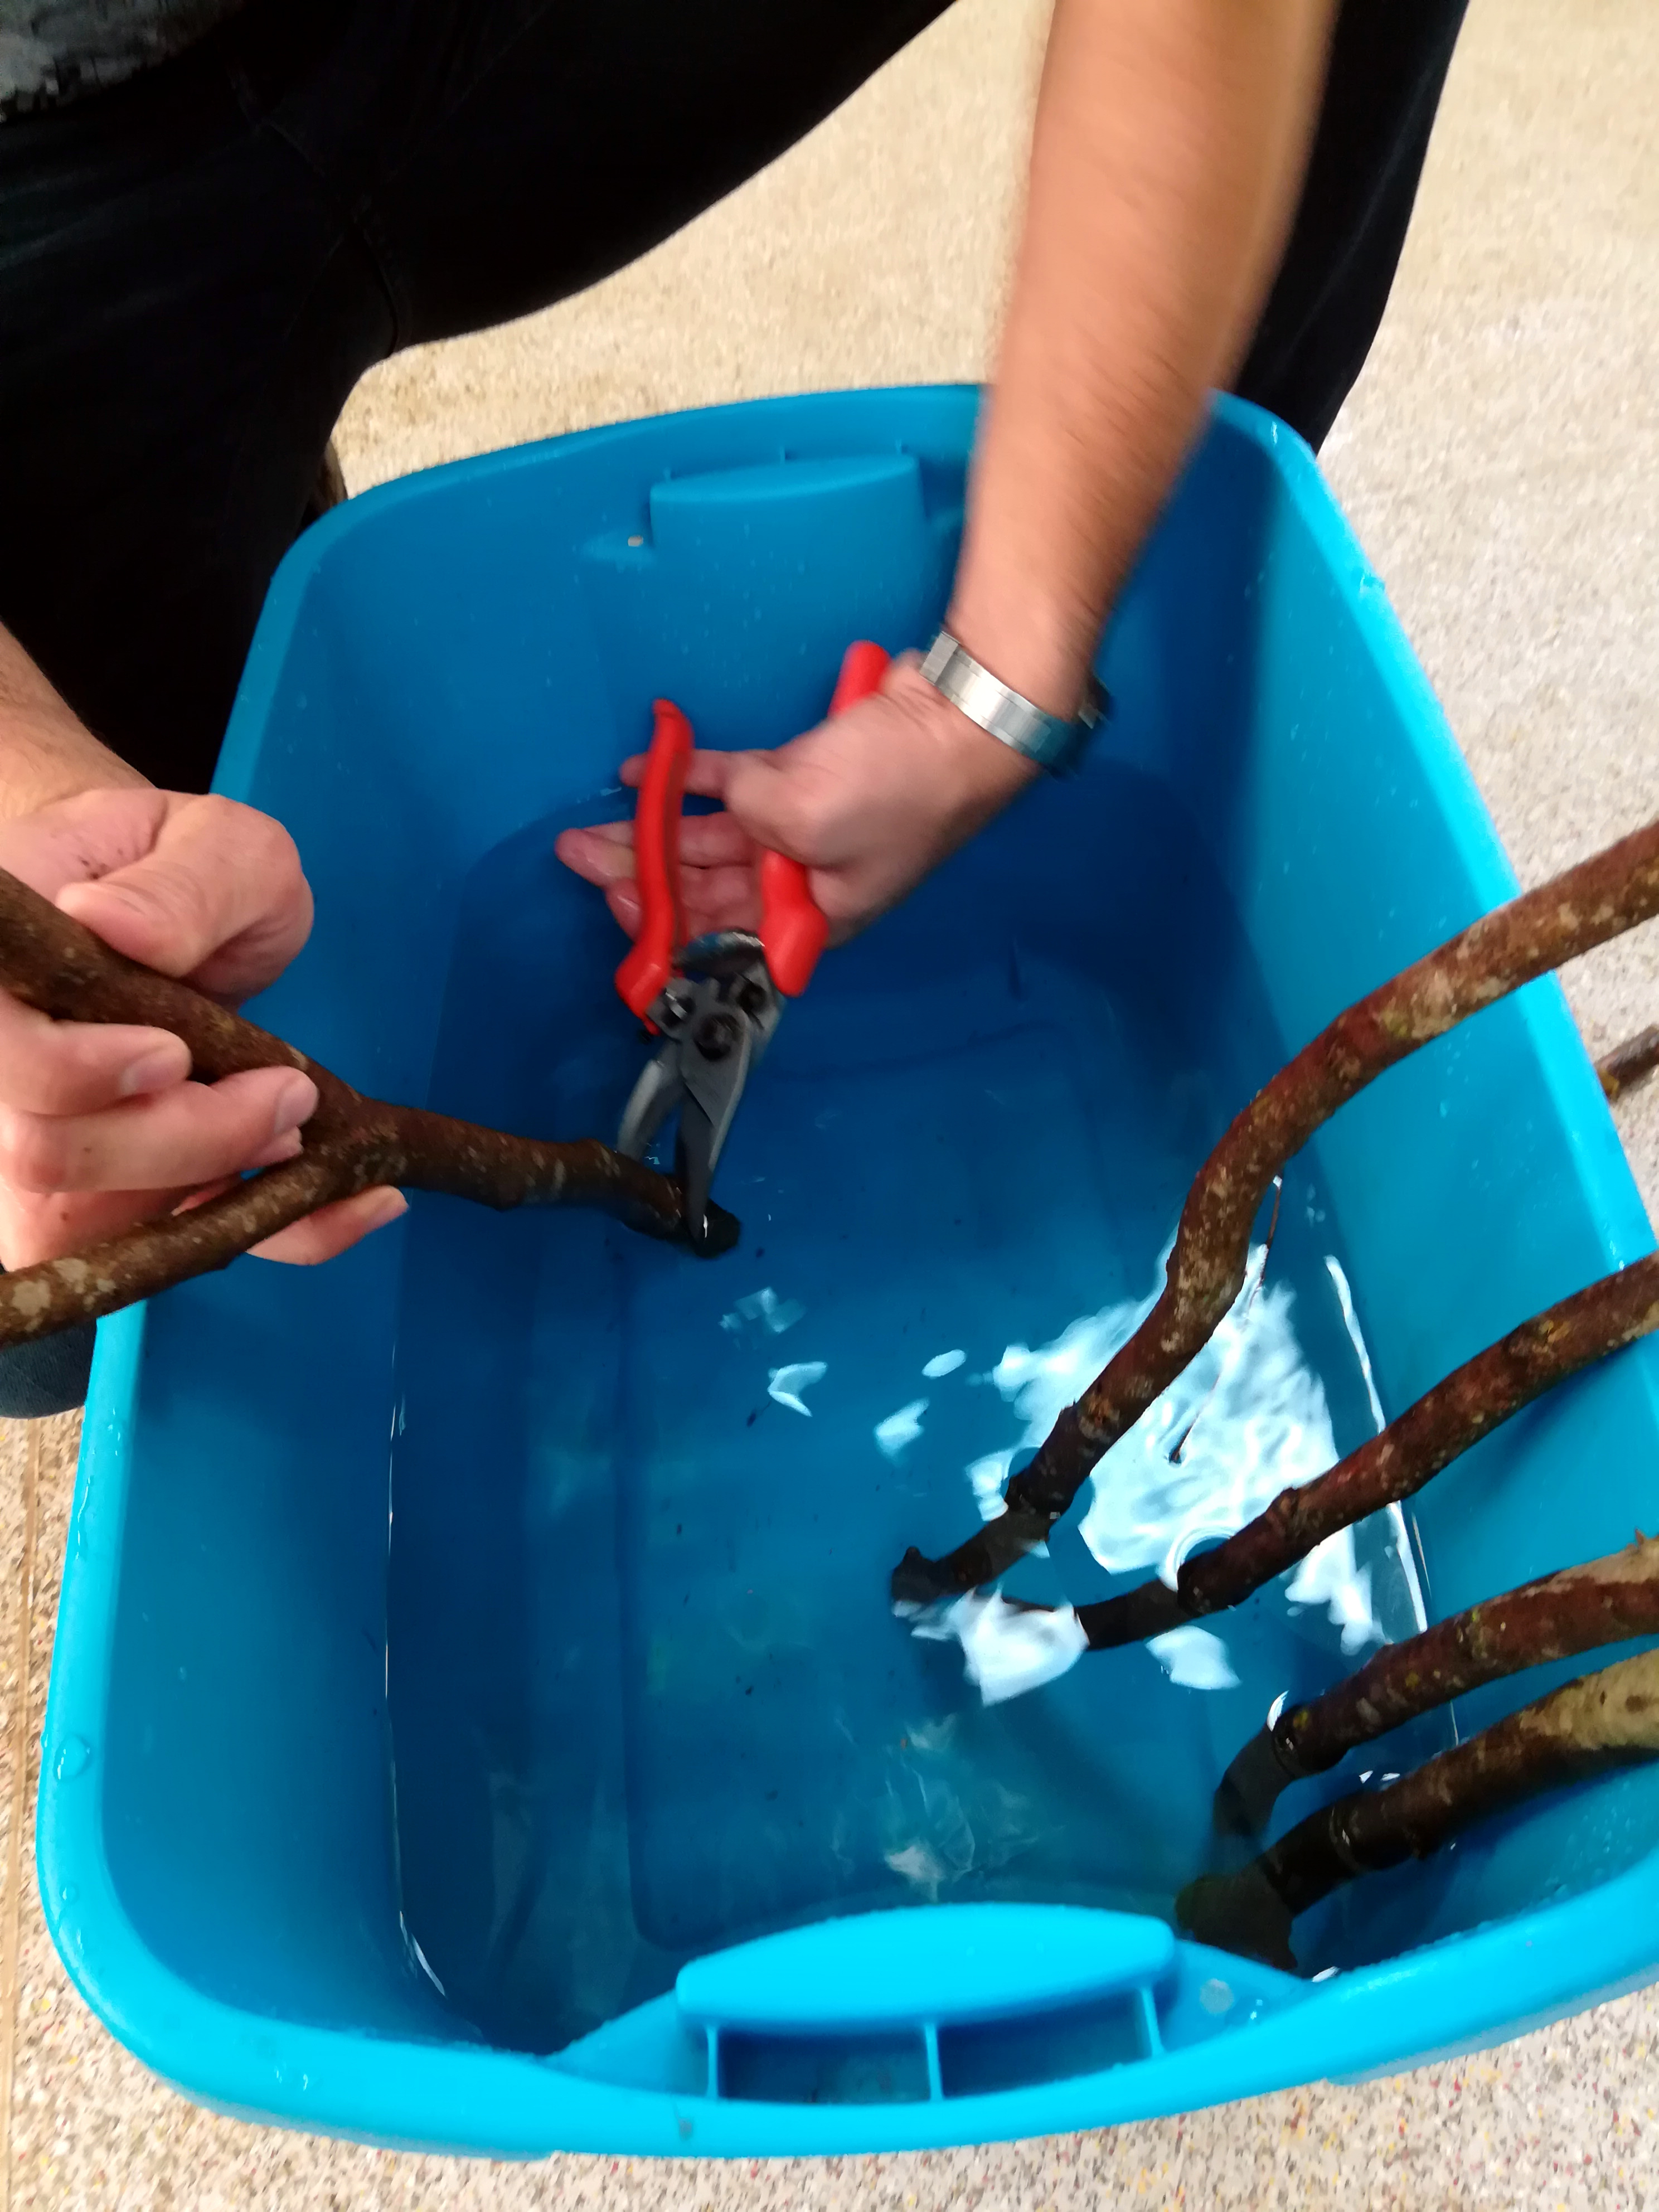
\includegraphics[width = \tw]{pictures/recutting.jpg}}
\end{minipage}
\begin{minipage}{0.6\tw}
	\begin{itemize}[<+->]
		\item Si no se colecta antes del amanecer, hay que \textbf{rehidratar} las muestras por una noche en un cubo de agua en una bolsa de plástico
		\item \textbf{Cortar} la parte basípeta de la muestra bajo agua
	\end{itemize}	
\end{minipage}	
\end{frame}

\begin{frame}
\frametitle{Deshidratación en la mesa de laboratorio}
\only<1>{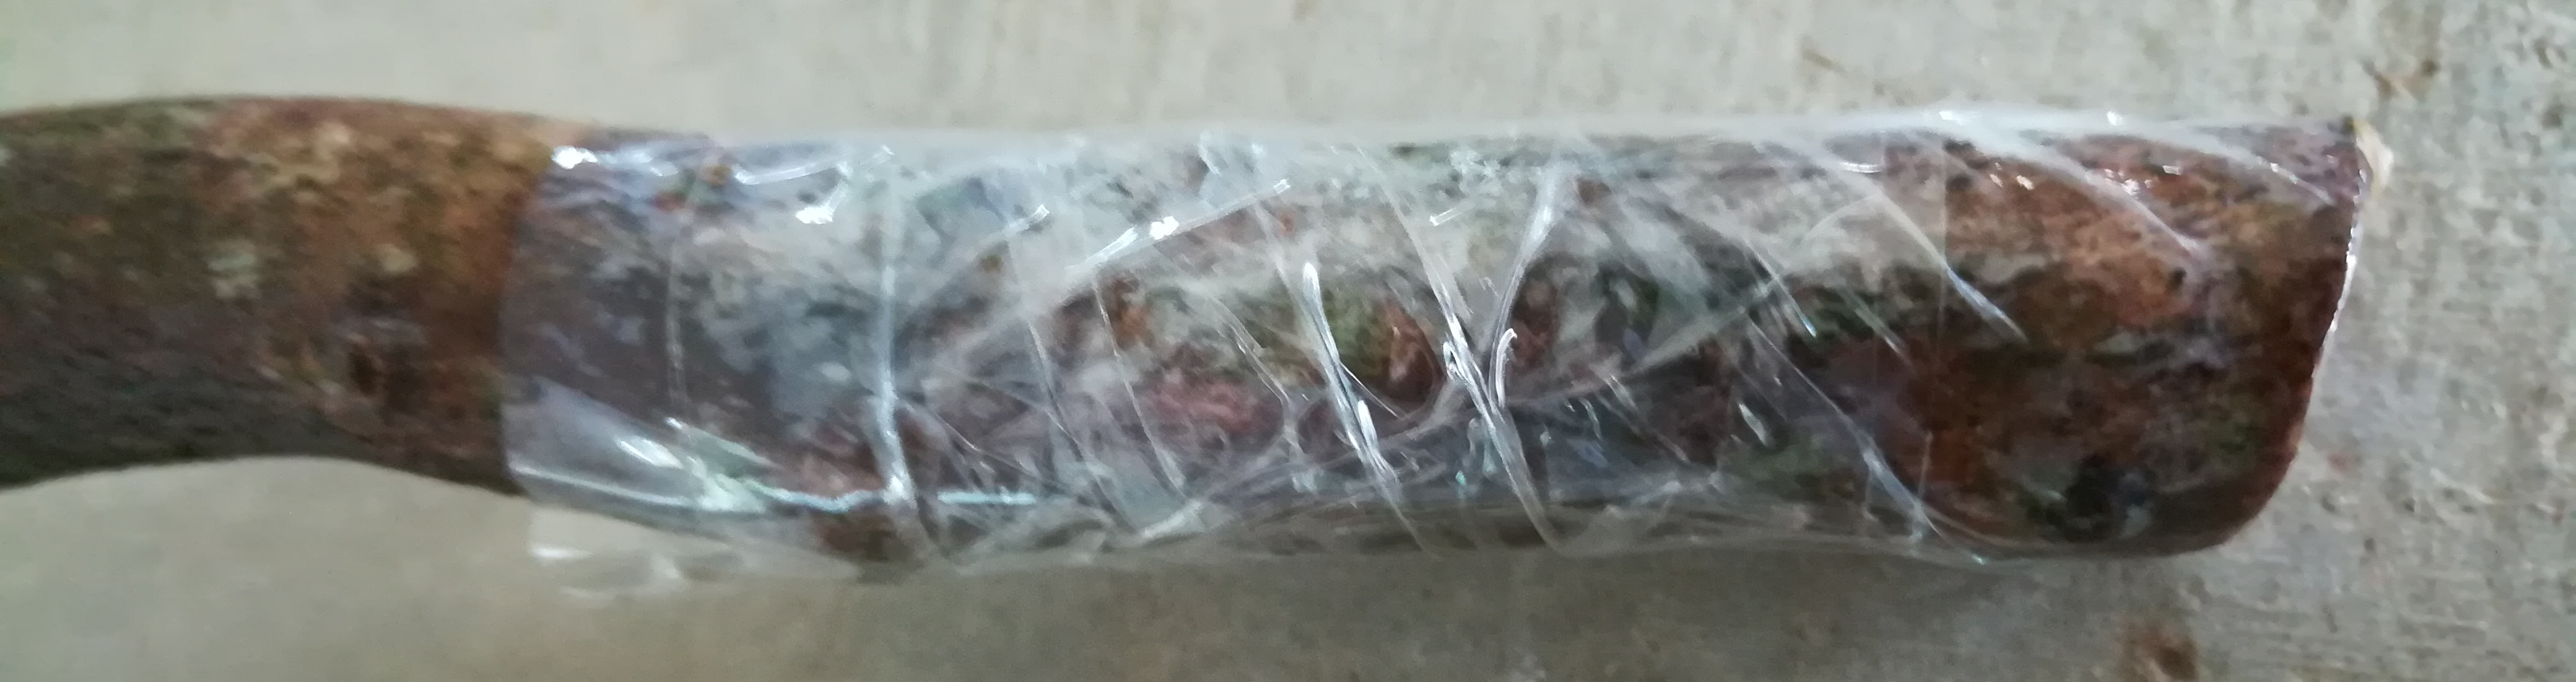
\includegraphics[width = \tw]{pictures/wrapping.jpg}}
\only<2->{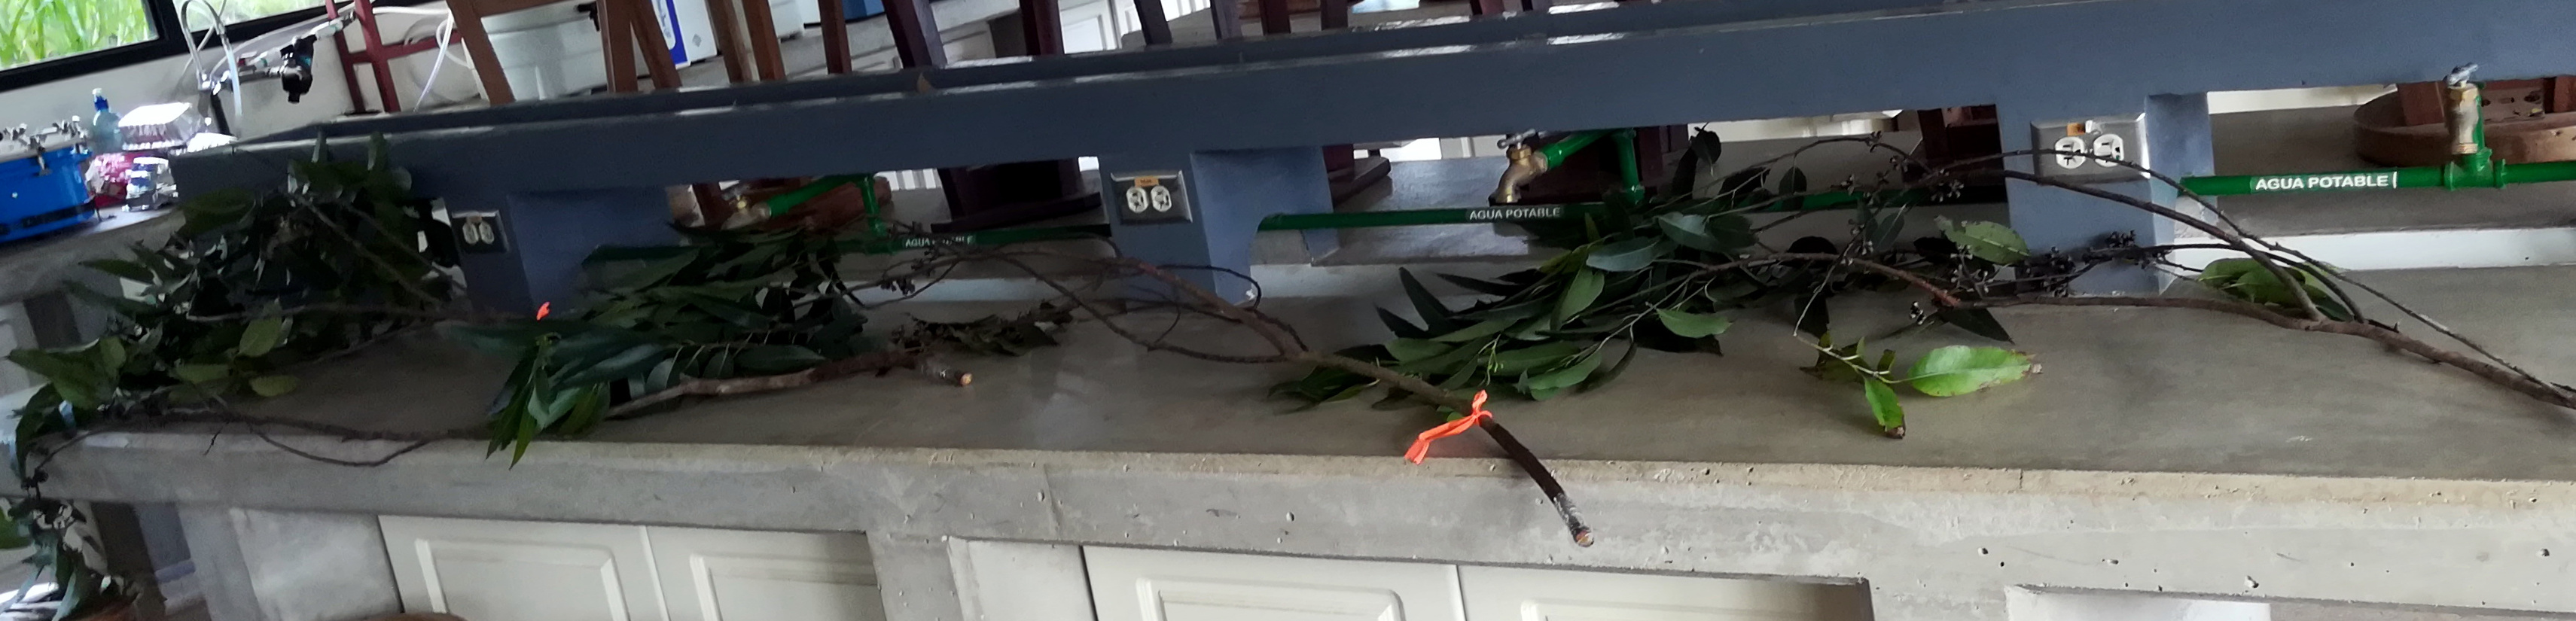
\includegraphics[width = \tw]{pictures/bench_drying1.jpg}}
\begin{itemize}[<+-| alert@+>]
  \item Después de tomar las muestras del agua, enrollar lado basípeto de las muestras en Parafilm o película de plástico
  \item Secar las muestras por tiempos diferentes (entre 1h y varios días) para llegar a potenciales de agua diferentes
  \item Guardar una muestra completamente saturada para el potencial hídrico inicial
\end{itemize}	
\end{frame}



\begin{frame}
	\frametitle{Preparación de muestras para potenciales hídricos}
\begin{changemargin}{-2em}{-2em}
\begin{minipage}{0.5\paperwidth}
  \begin{itemize}[<+-| alert@+>]
    \item Escoger una rama en buen estado
    \item Envolver rama en papel de aluminio
	\item Poner rama en bolsa de plástico
	\item Poner muestra entera en bolsa de plástico grande con papel ligeramente mojado para permitir que se equilibre la presión (por lo menos una hora)
  \end{itemize}	
\end{minipage}	
\quad\
\begin{minipage}{0.4\paperwidth}
  \centering
  \only<1>{
	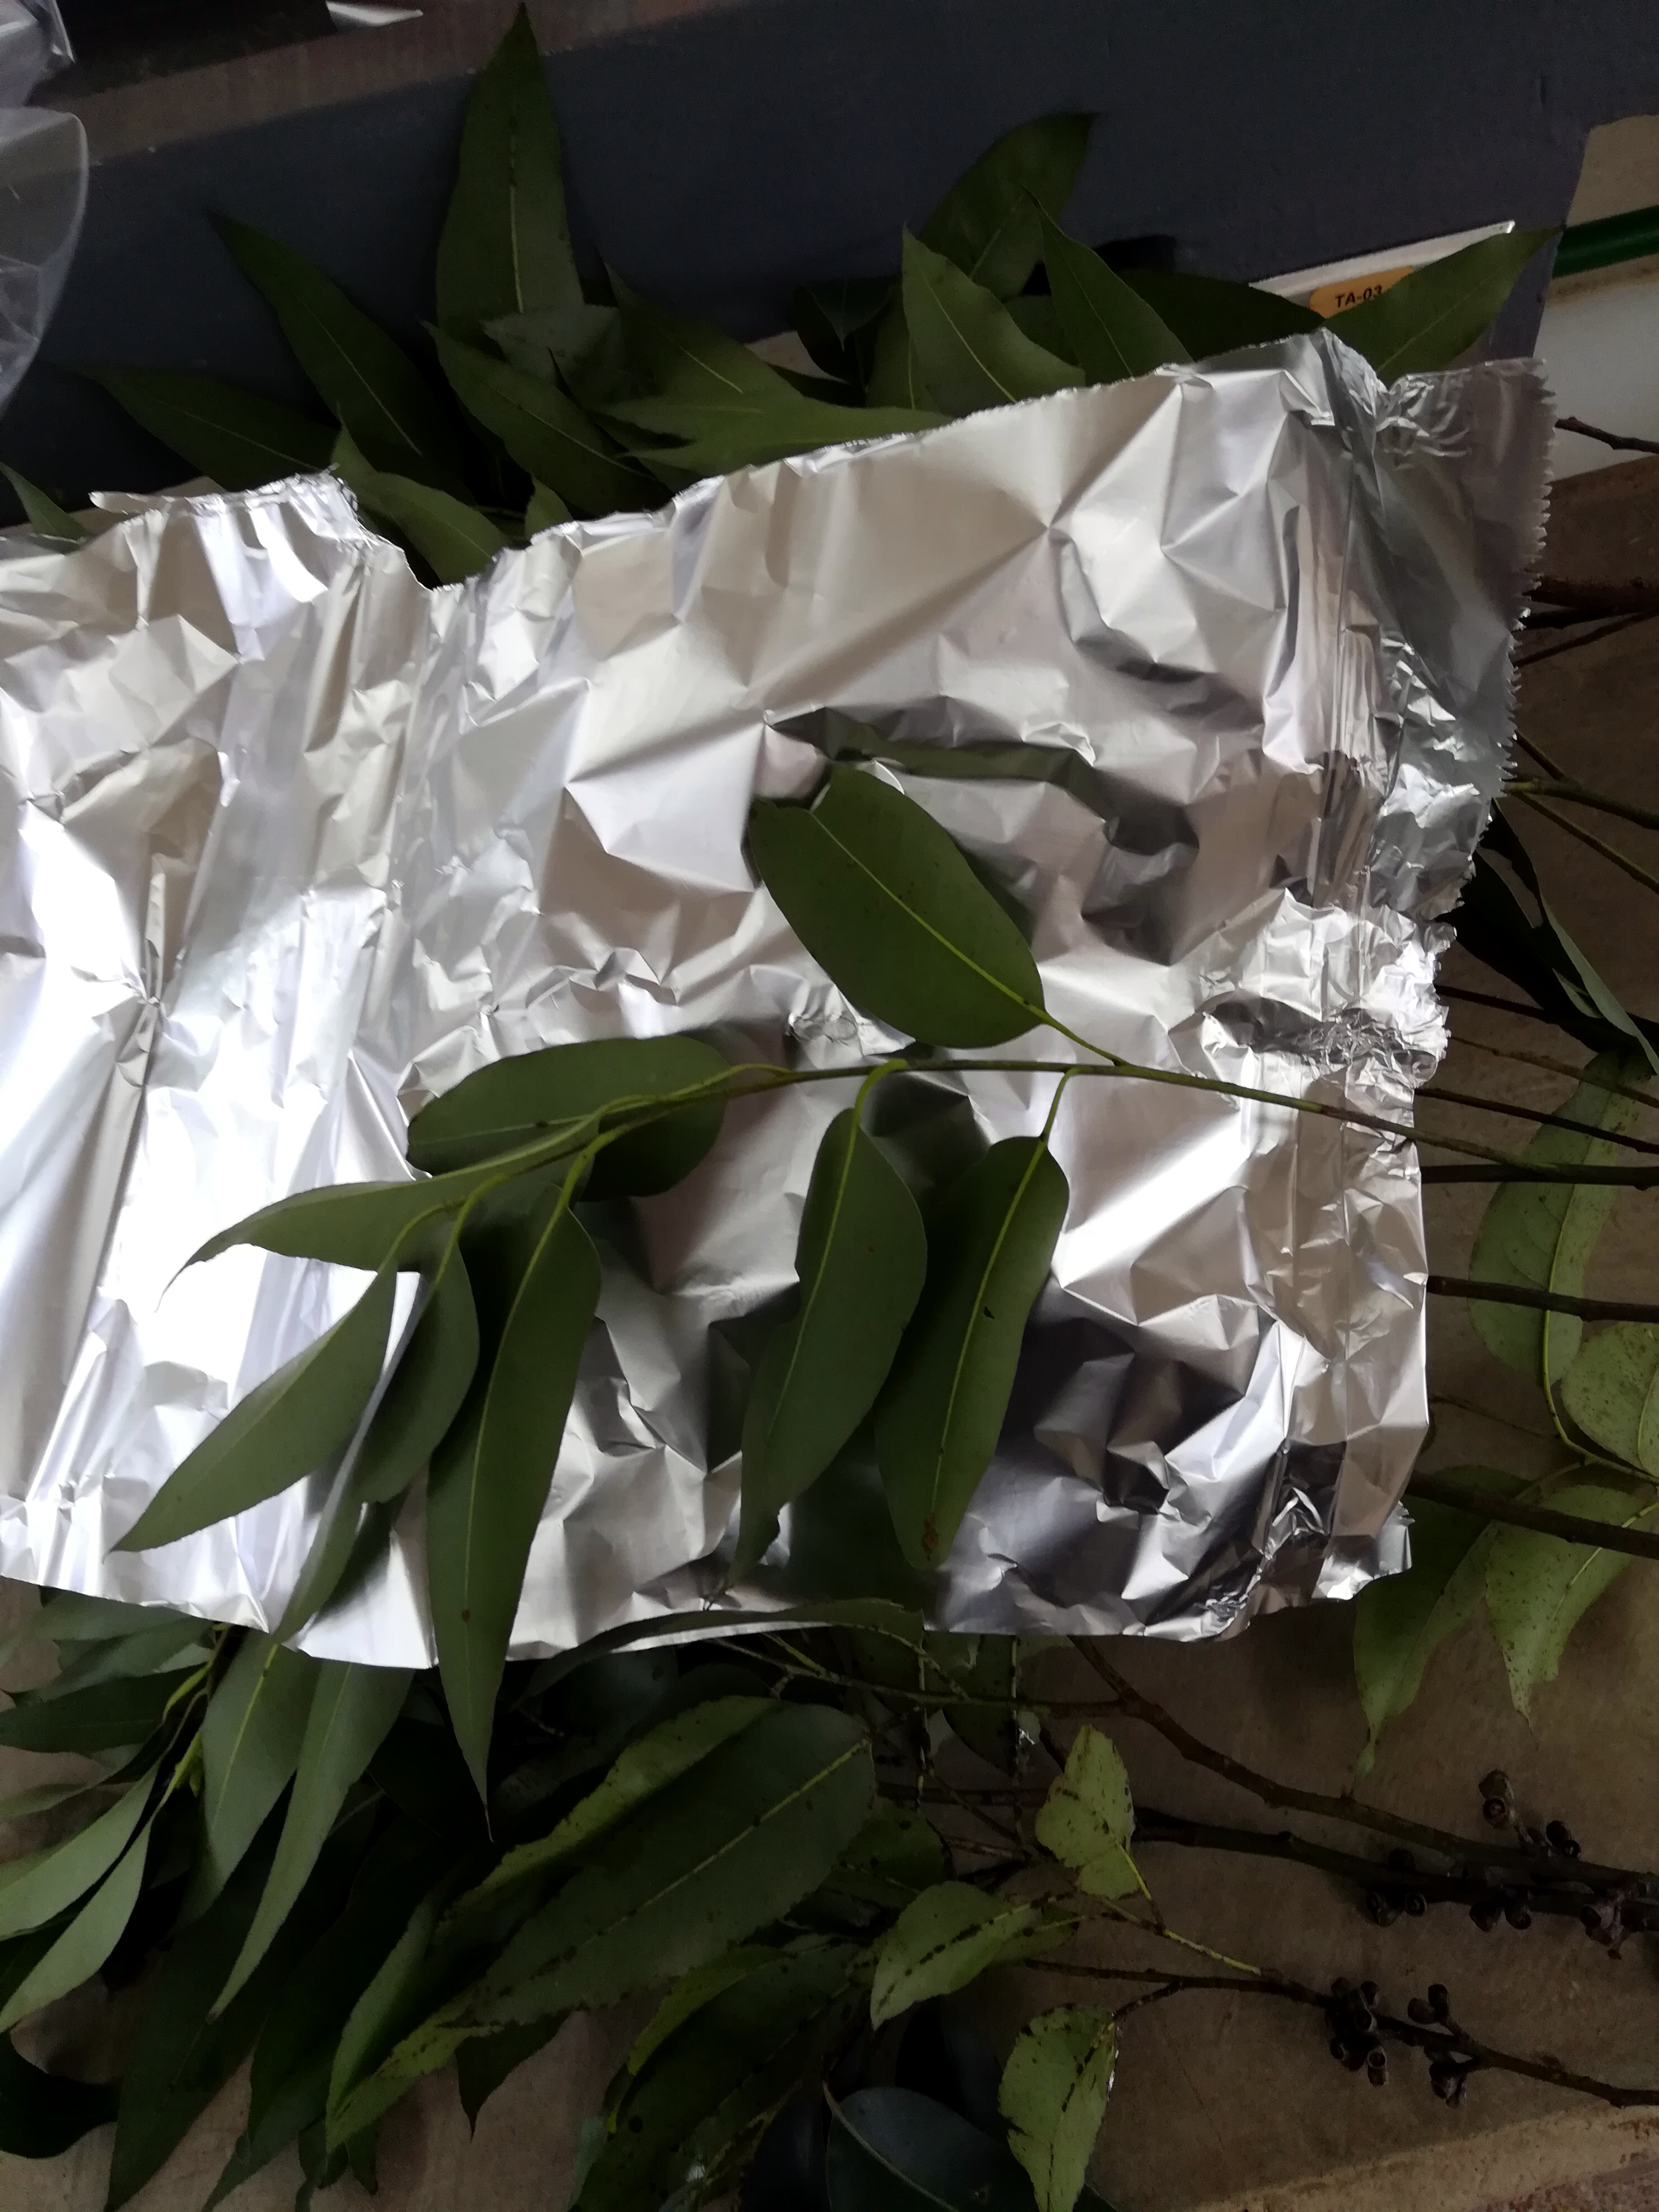
\includegraphics[width = \tw]{pictures/leaf_prep1.jpg}}
  \only<2>{
	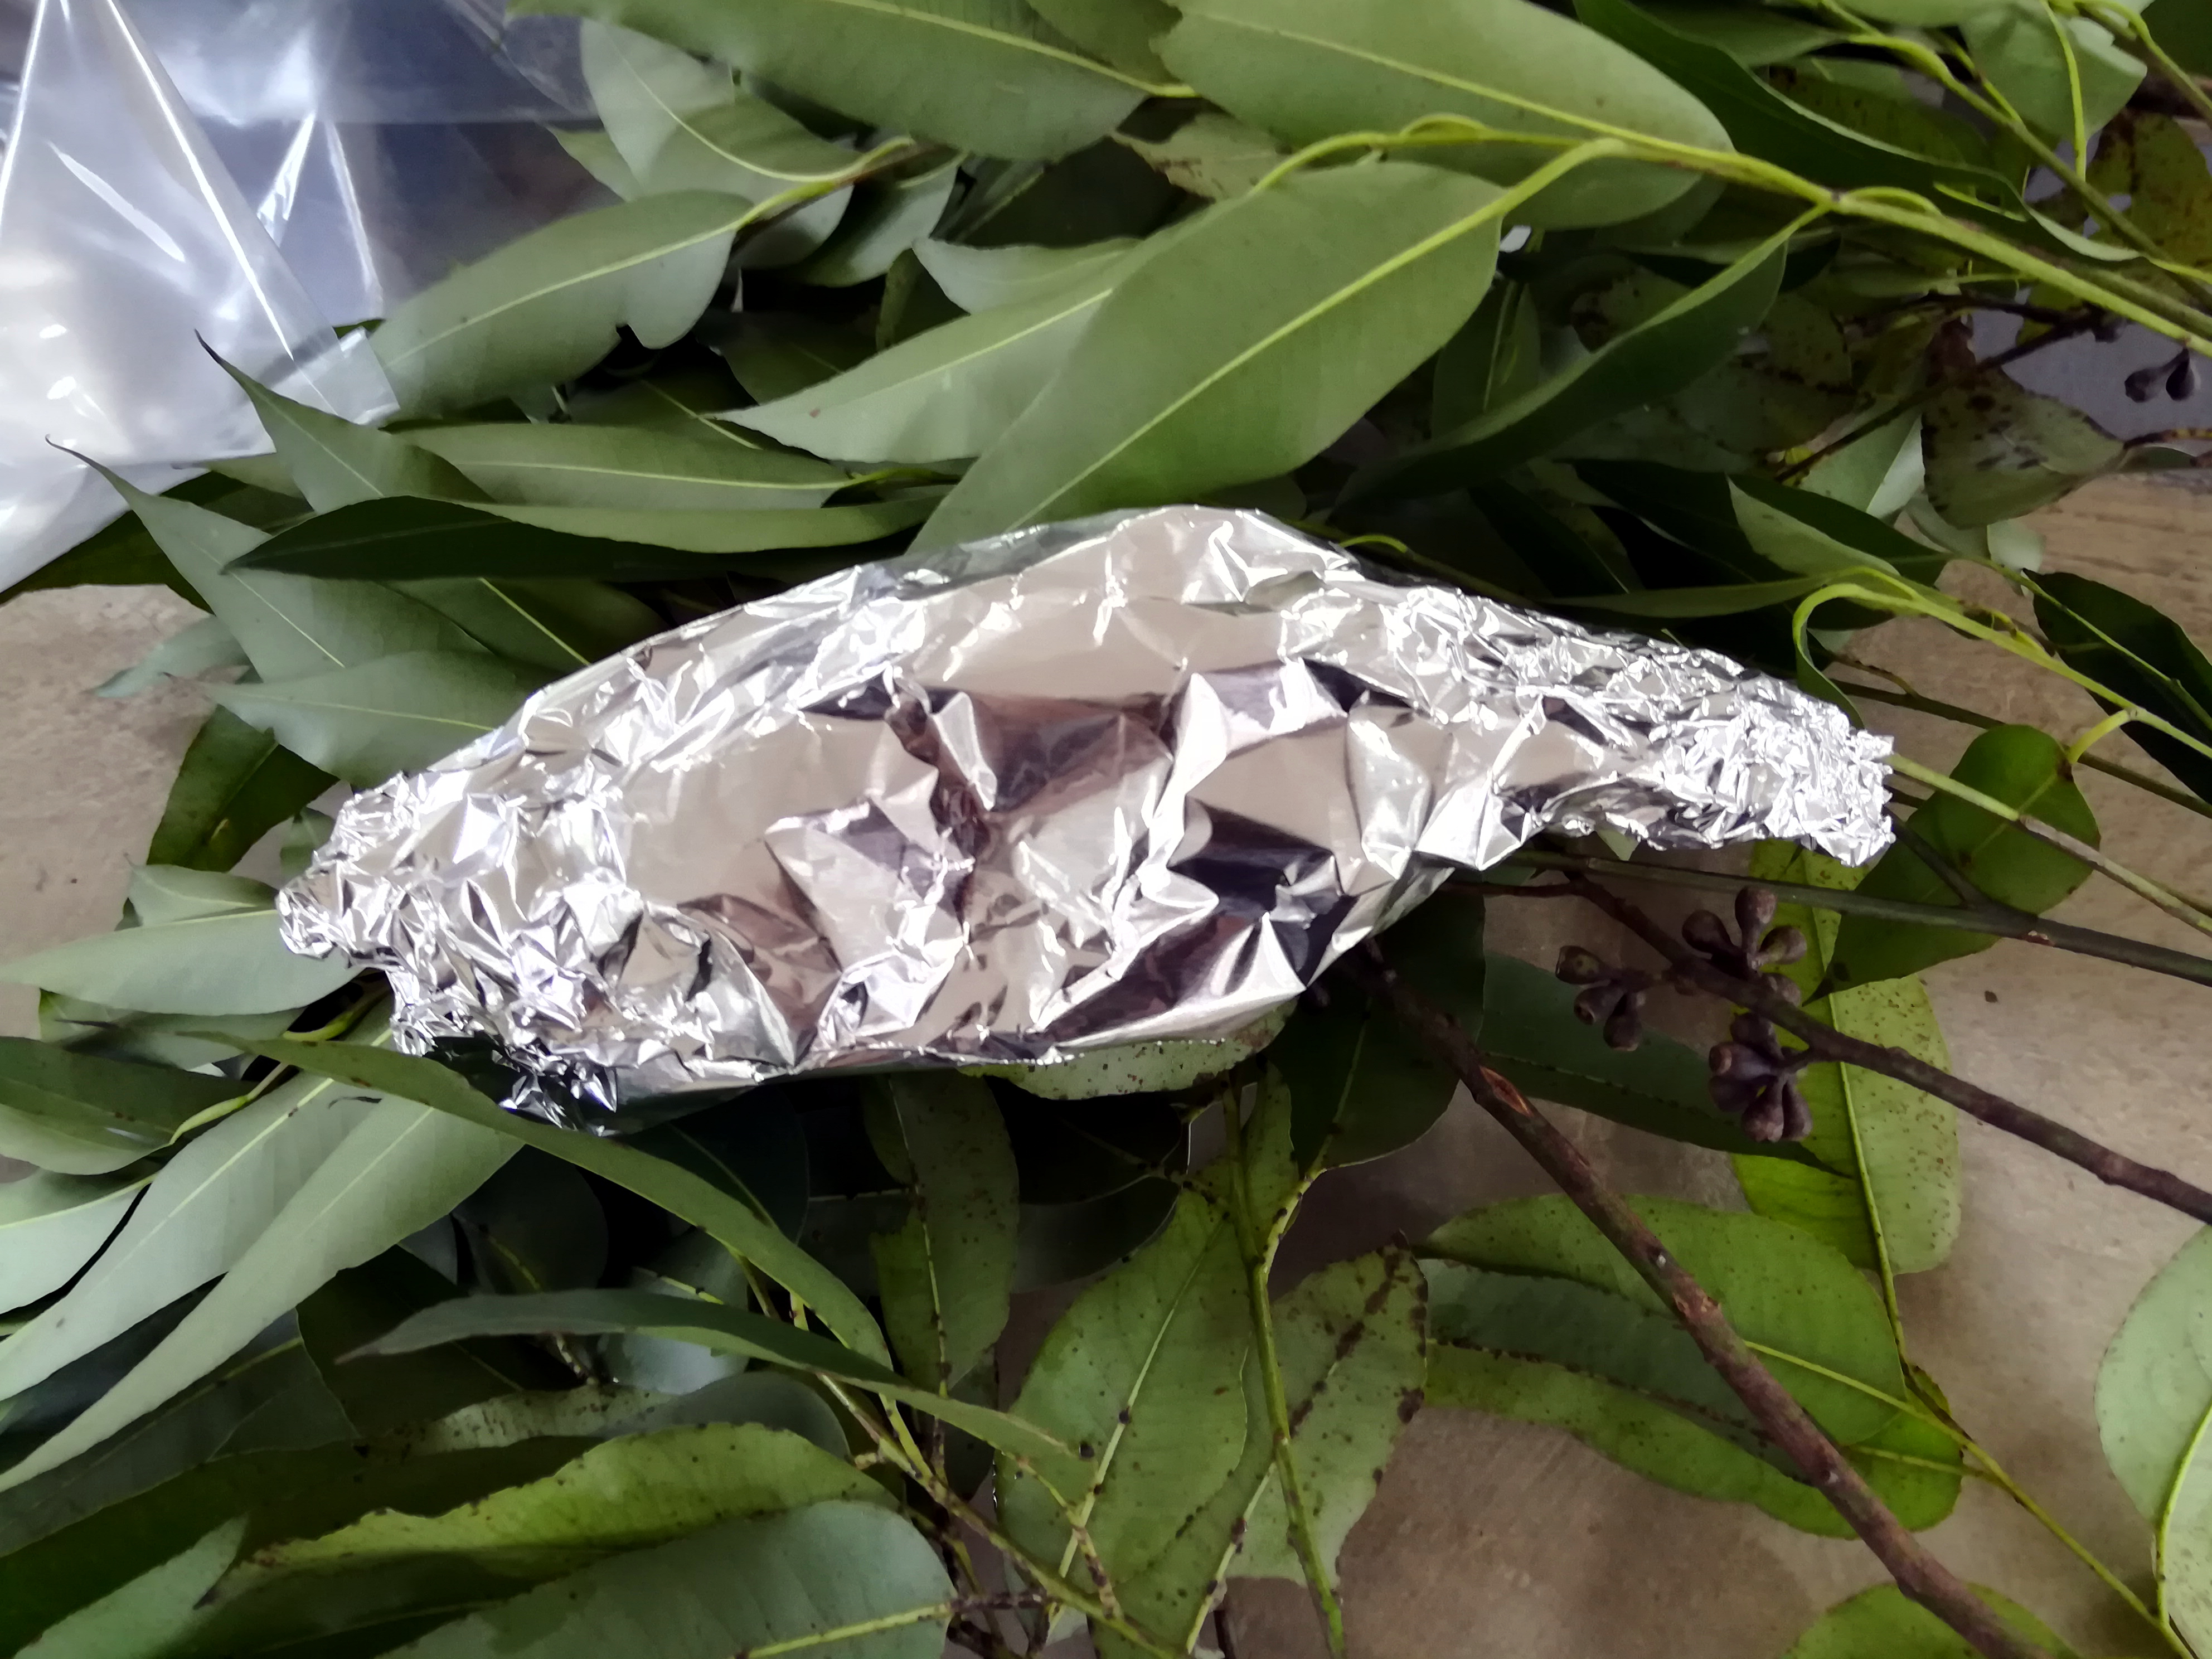
\includegraphics[width = \tw]{pictures/leaf_prep2.jpg}}
  \only<3>{
	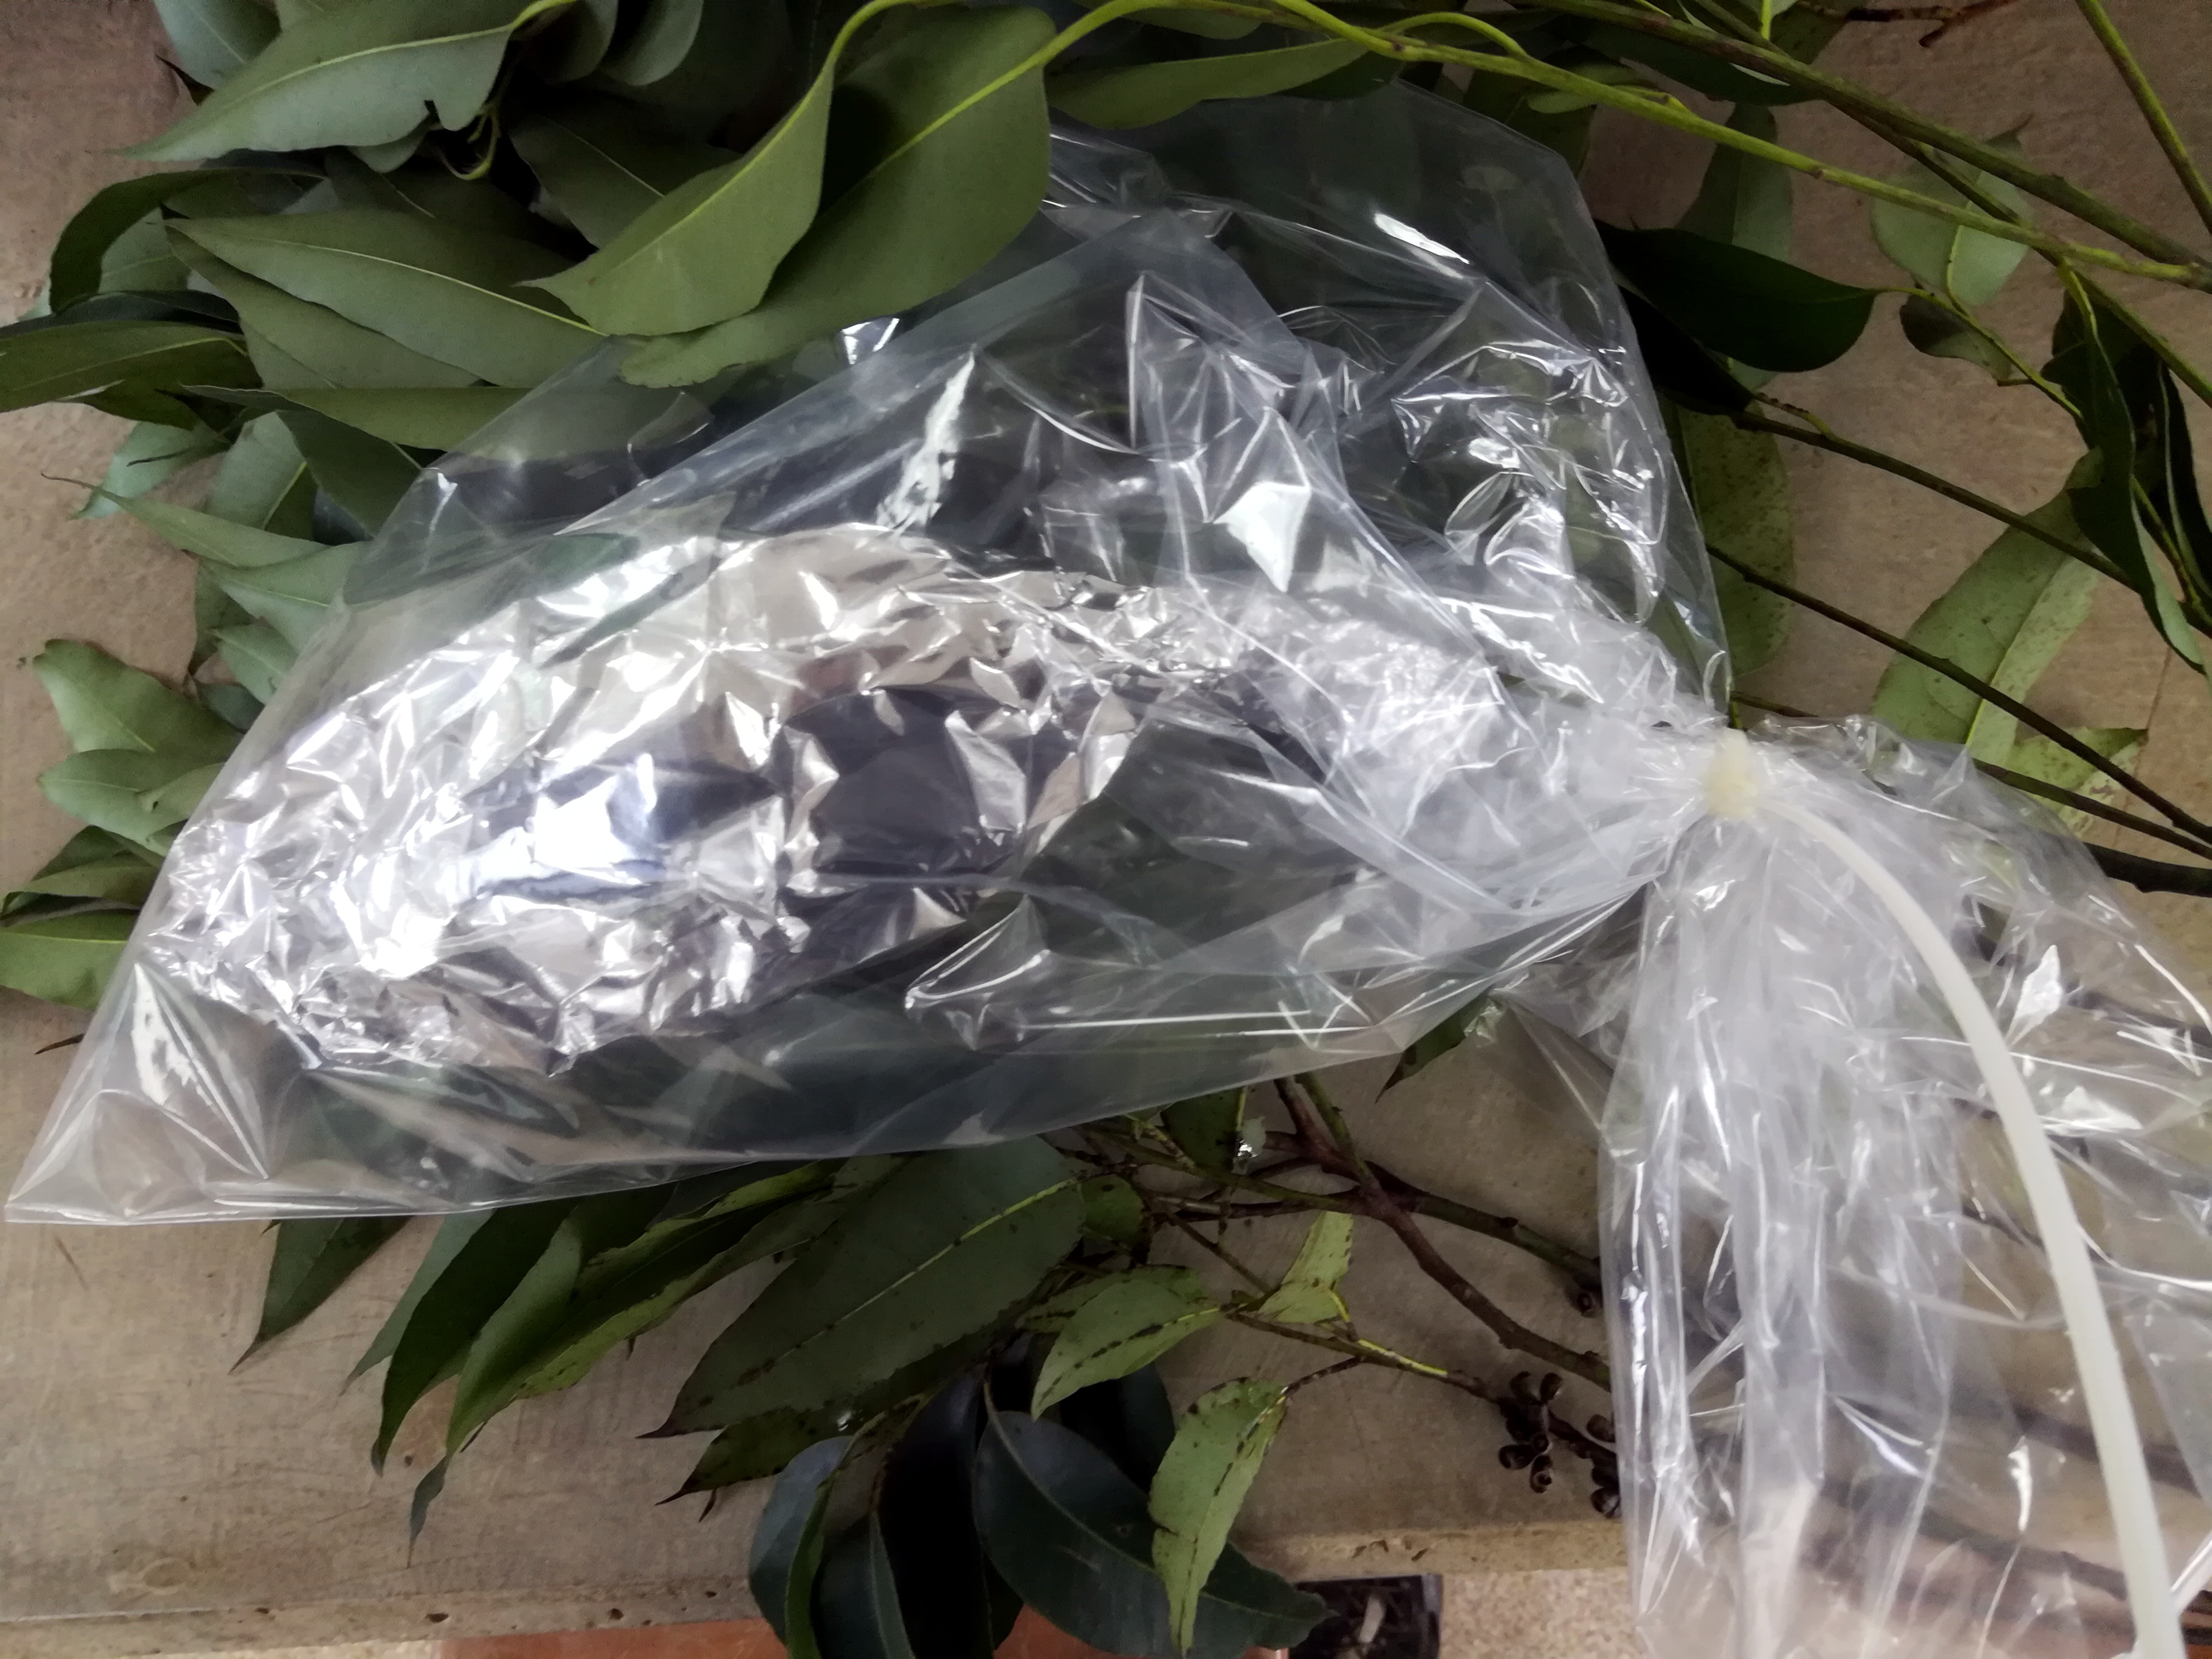
\includegraphics[width = \tw]{pictures/leaf_prep3.jpg}}
  \only<4>{
	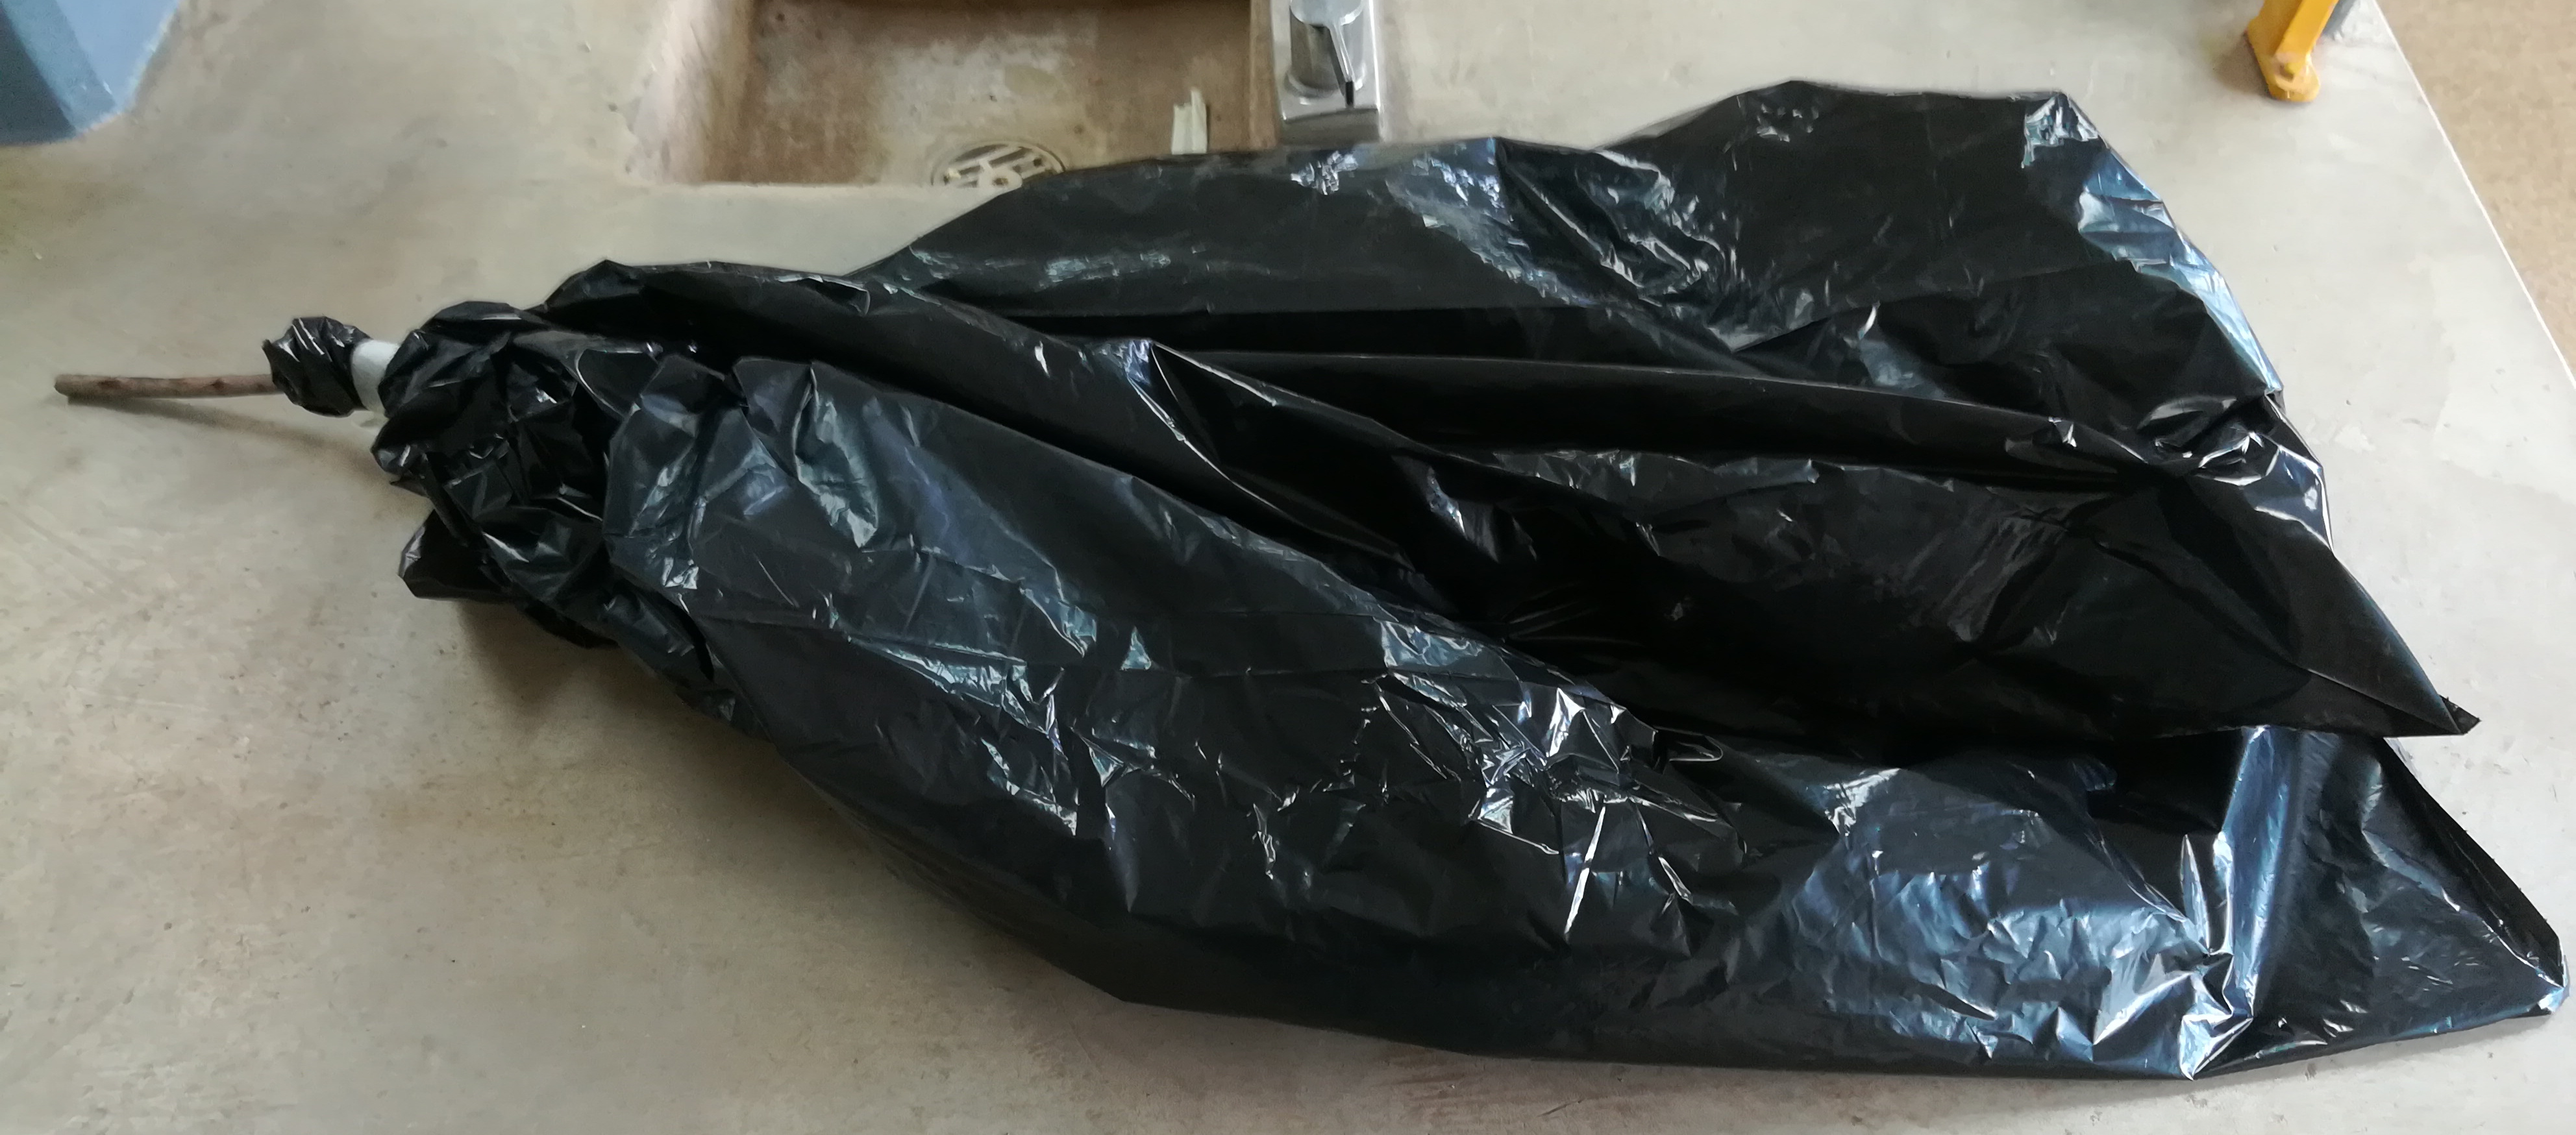
\includegraphics[width = \tw]{pictures/leaf_prep4.jpg}}
\end{minipage}
\end{changemargin}
\end{frame}

\begin{frame}
\frametitle{Medición de potenciales hídricos}
\centering{	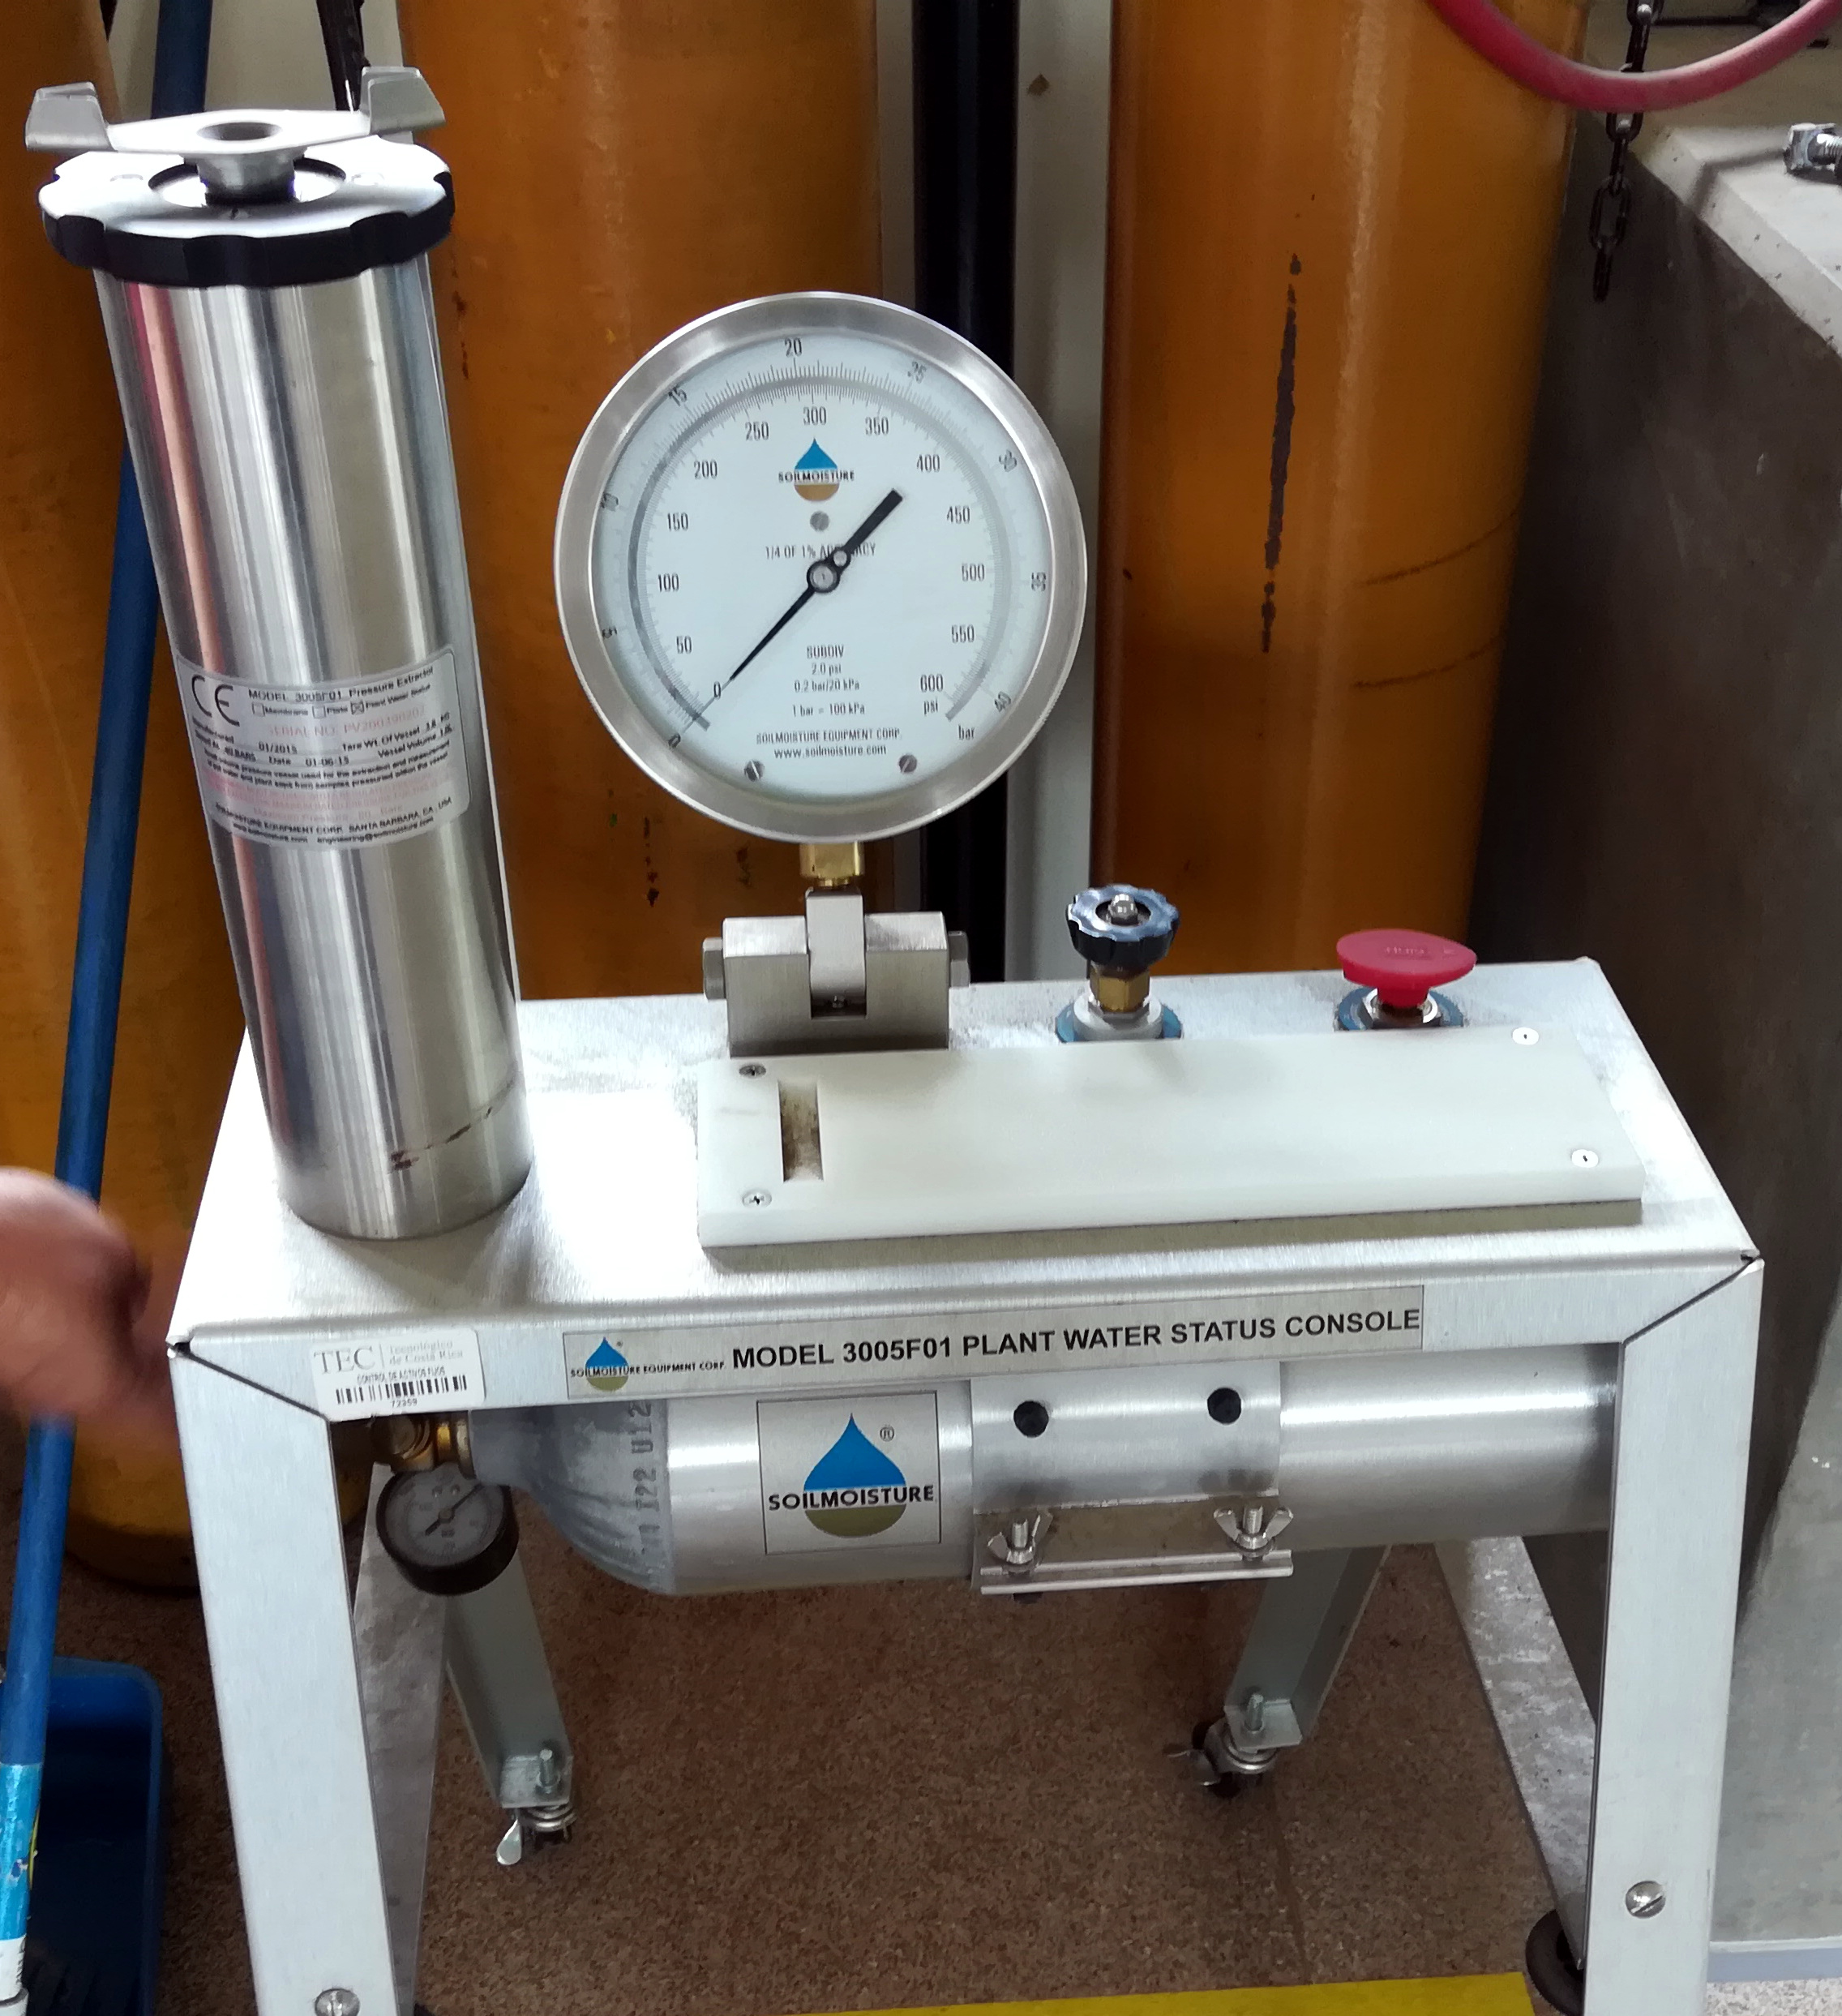
\includegraphics[height =0.4\tw]{pictures/bomba1.jpg}
			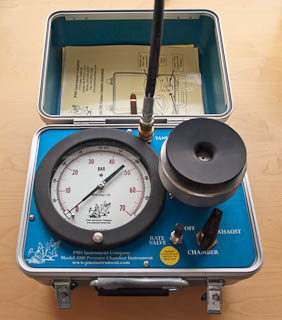
\includegraphics[height =0.4\tw]{pictures/bomba2.jpg}}
\begin{itemize}[<+->]
  \item Medición sigue el protocolo discutido antes del almuerzo
  \item Es recomendable medir potenciales de \alert<2>{2--3 hojas de cada submuestra}
\end{itemize}	
\end{frame}


\begin{frame}
\frametitle{Preparación de muestras para XylEm Plus}
\centering
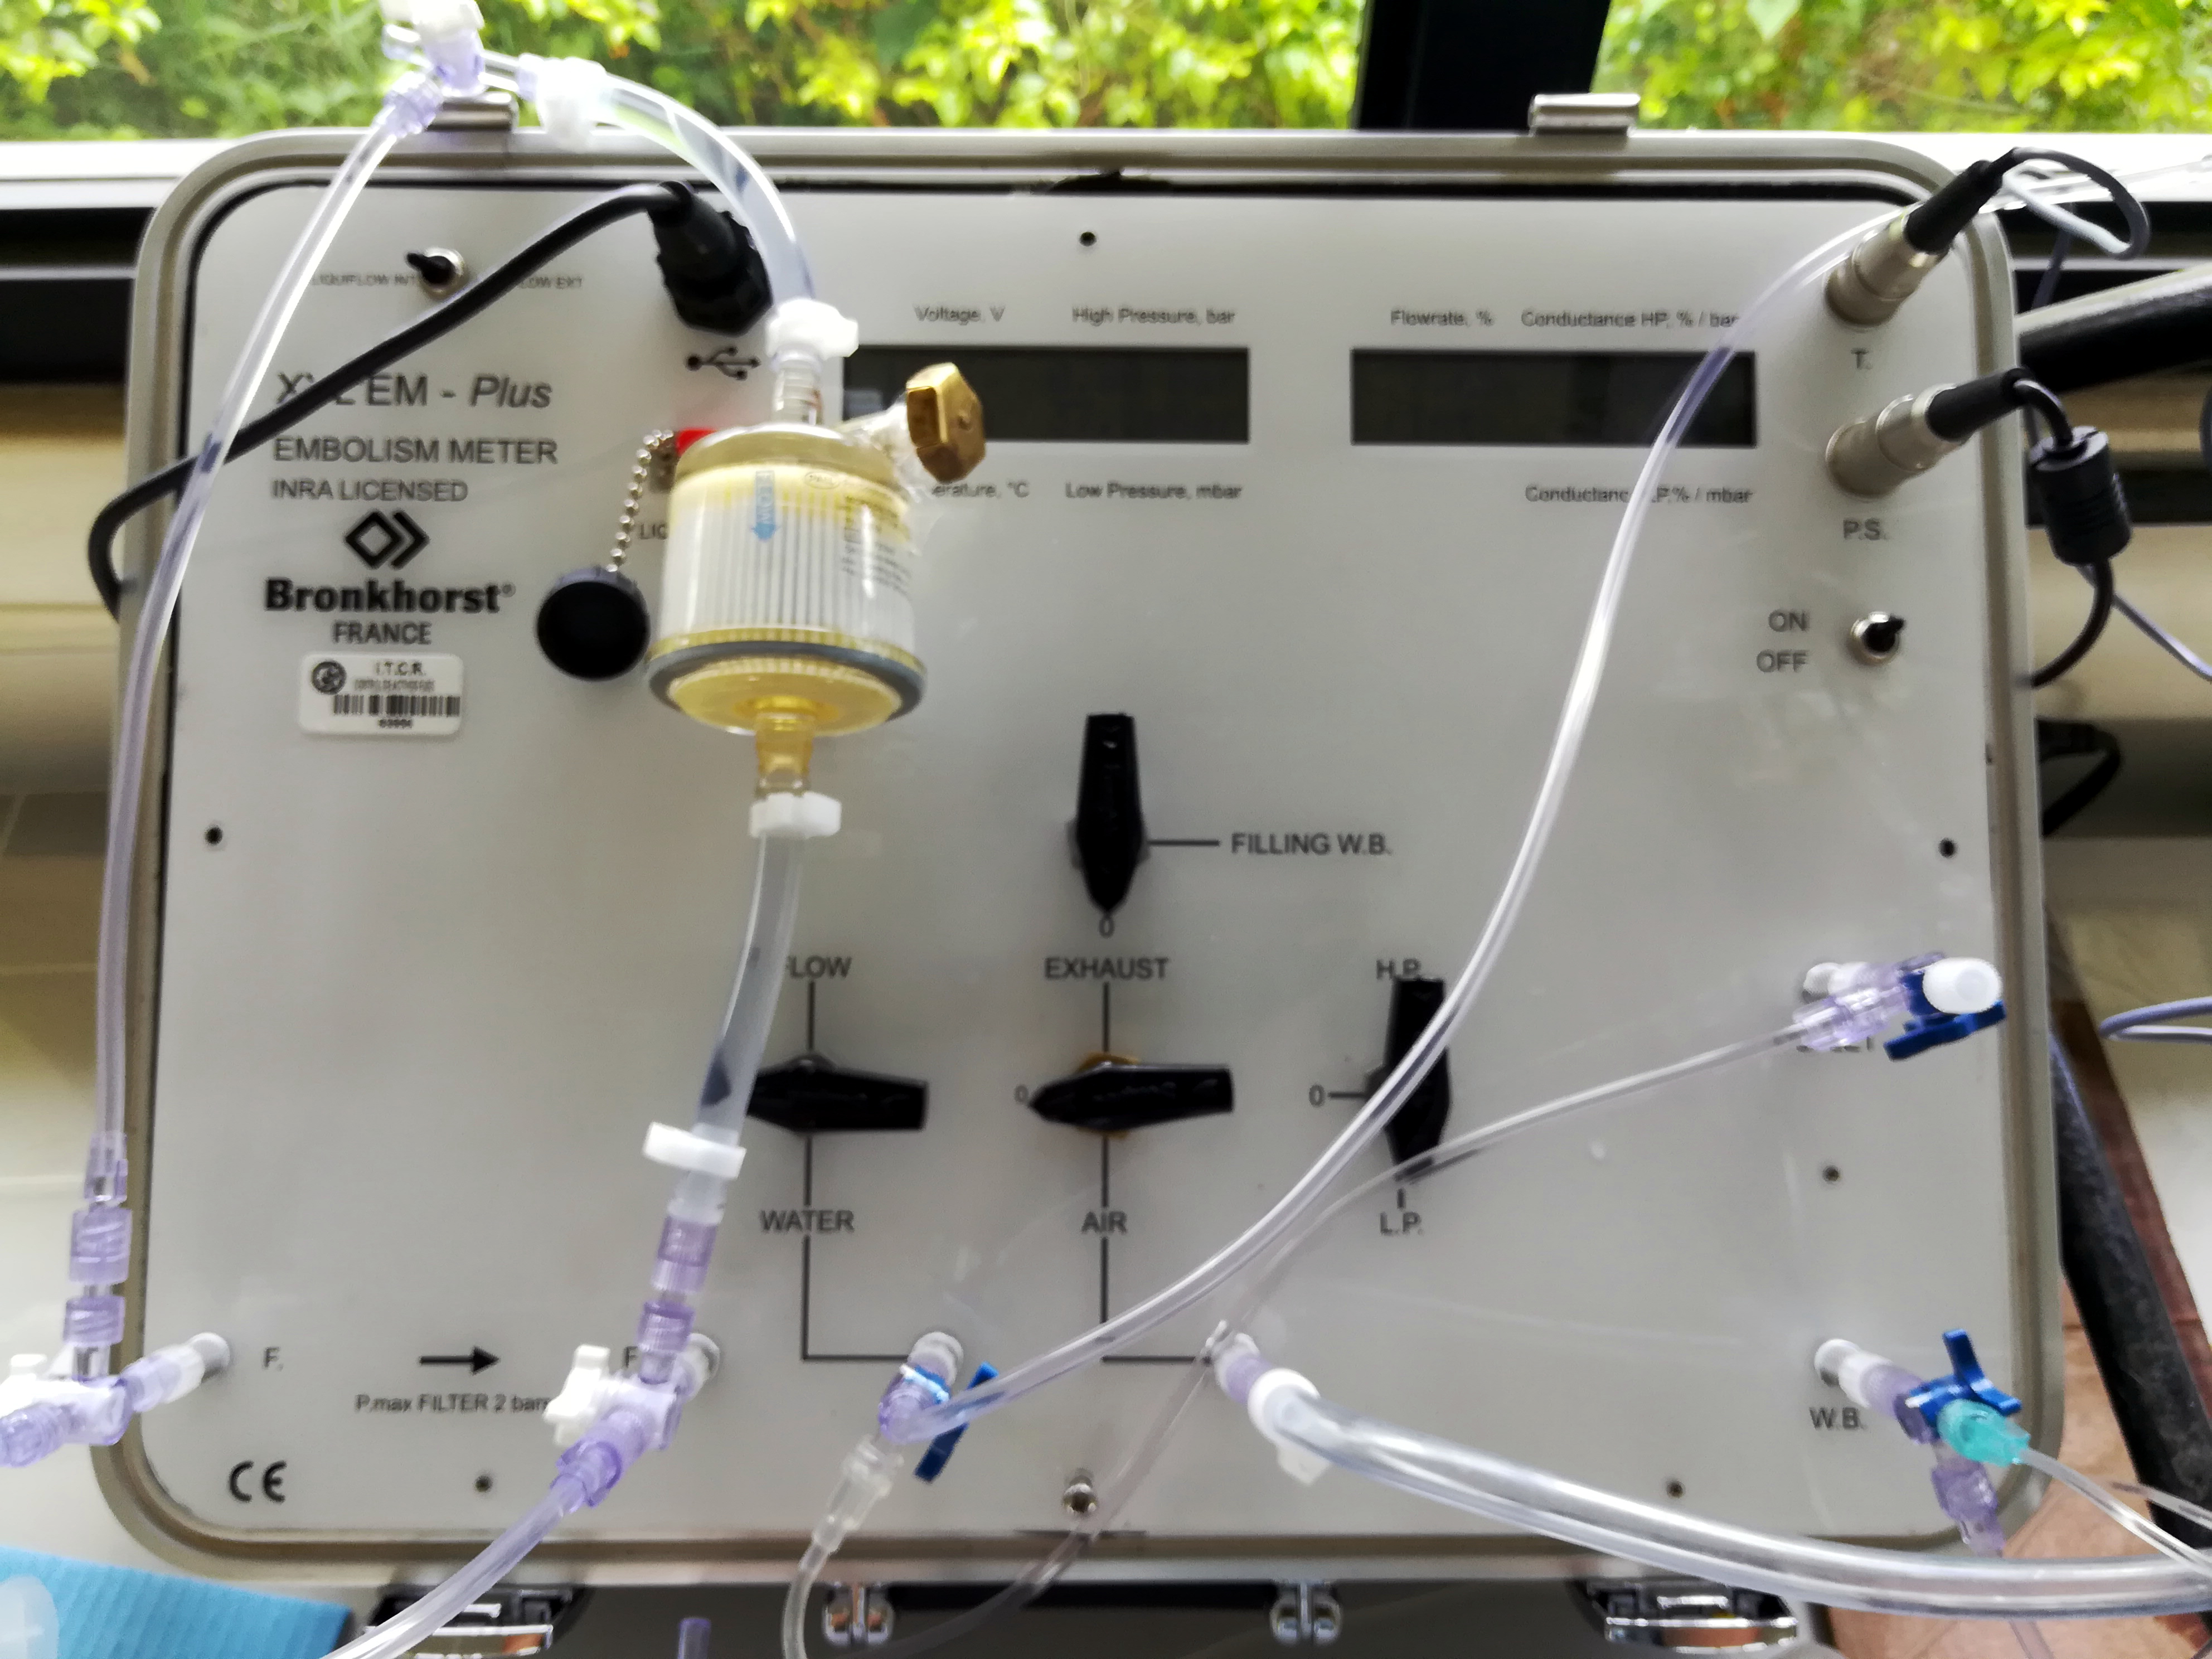
\includegraphics[width =0.4\tw]{pictures/xylem.jpg}
\begin{itemize}[<+->]
  \item Cortar muestras bajo agua con una cuchilla
  \item Recortar varias veces
  \item Muestras para PLC pueden ser mucho más pequeñas que para conductividad específica 
  \begin{itemize}
    \item<3>[\rar] Fracción de vasos embolizados por unidad de área queda igual  
    \item<3| alert@3>[\rar] Recomendado: 3--10 cm de largo, 3--10 mm de diámetro
  \end{itemize}
\end{itemize}	
\end{frame}

\begin{frame}
\frametitle{Conección de muestras}
\begin{minipage}{0.38\tw}
 \centering
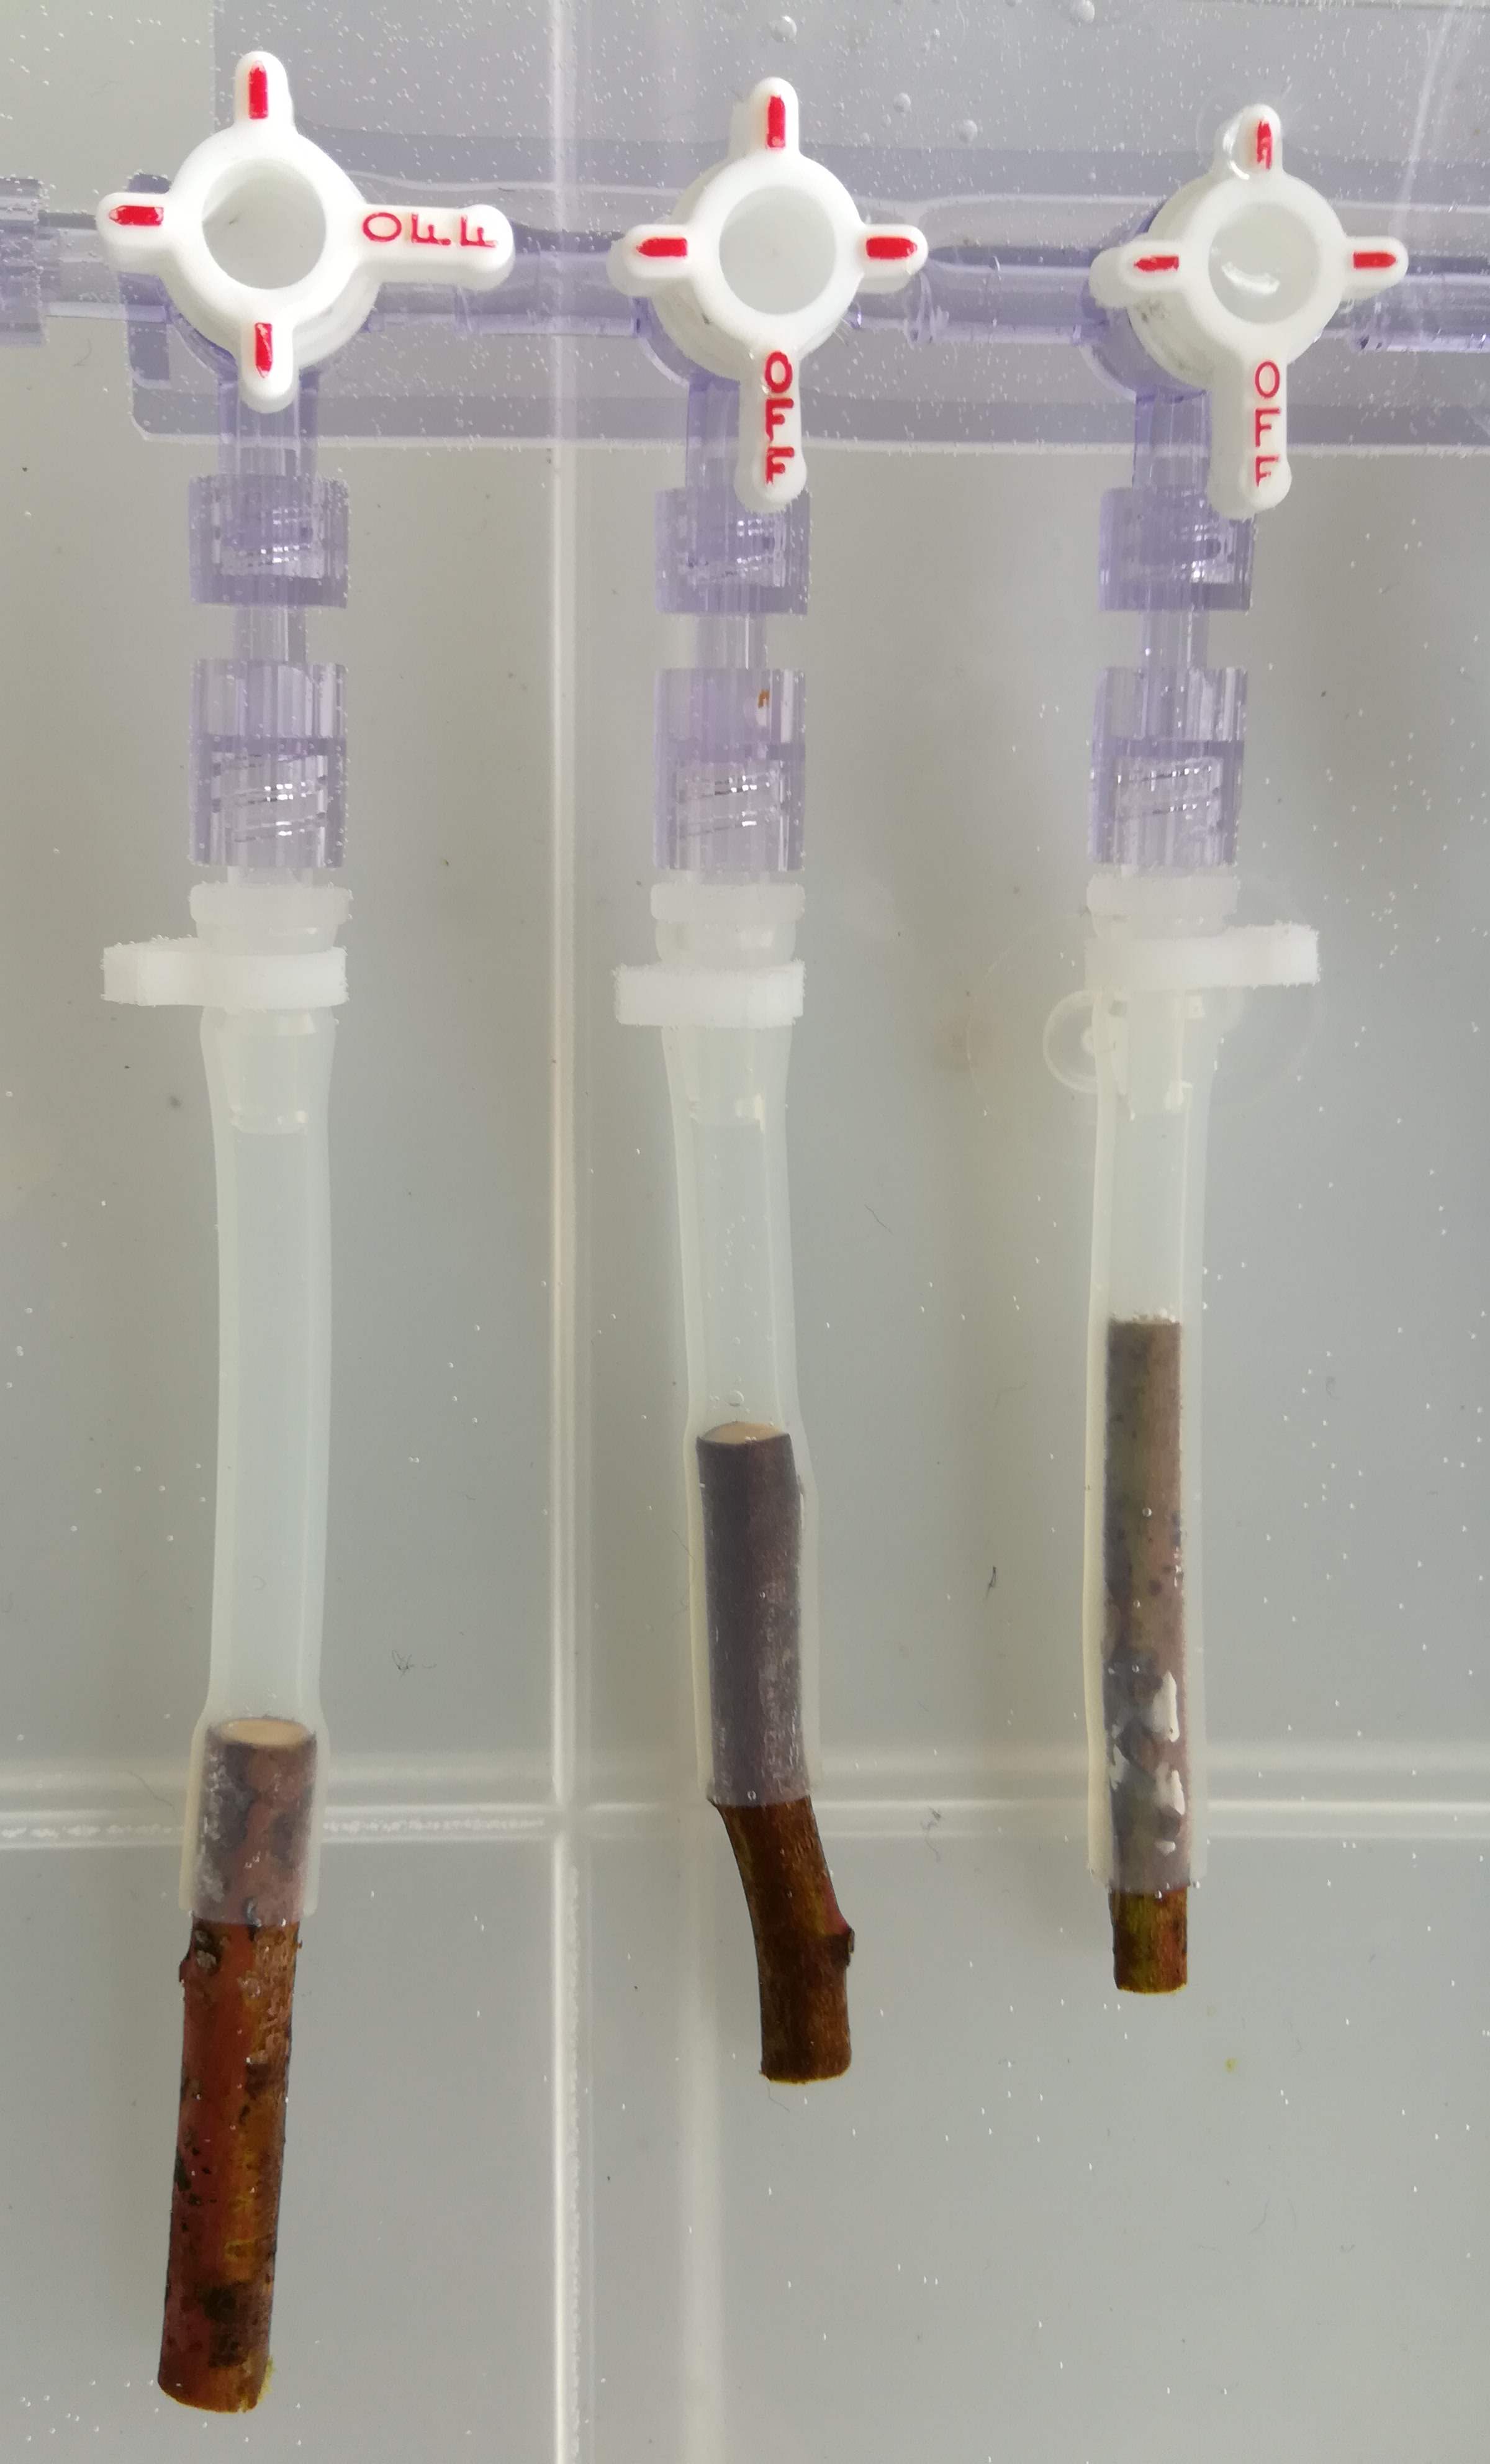
\includegraphics[width = \tw]{pictures/connecting.jpg}
\end{minipage}
\begin{minipage}{0.6\tw}
\begin{itemize}[<+->]  
  \item \alert<1>{Conectar} con tubos de XylEm \alert<1>{bajo agua} (hay que tener mucho cuidado a no desplazar embolías)
  \item \alert<2>{Quitar burbujas} usando una jeringa con solución de medición
  \item Es recomendable tomar \alert<3>{2--3 replicados por submuestra}
\end{itemize}	
\end{minipage}
\end{frame}

\begin{frame}
\frametitle{Medición de porcentaje de perdida de conductividad}
\textbf{¡Todas las mediciones se lleva a cabo bajo agua!}
\begin{itemize}[<+->]
	\item[\blue{1)}] Poner XylEm en \textit{low pressure mode} y medir primer muestra hasta que el XylWin software indica que la conductancia esté constante \alert<1>{(\Rar\ equilibrio dinámico)}
	\item[\blue{2)}] Repetir paso \Blue{1)}\ para las otras muestras conectadas
	\item[\blue{3)}] Poner XylEm en \textit{high pressure mode} y enjuagar muestras por \alert<3->{\textbf{5 min}}
	\item[\blue{4)}]Repetir pasos \Blue{1)} y \Blue{2)}\ hasta que la conductancia no se cambia después de enjuagar la muestra
\end{itemize}	
\only<1-4>{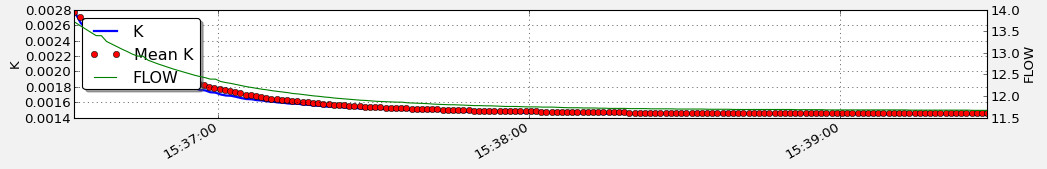
\includegraphics[width = \tw]{pictures/screenshot_detail.jpg}}
\only<5>{\alert{\textbf{Diferencias a protocolo estandar:}
\begin{itemize}
  \item Tiempo para enjuagar más corto
  \item Valor inicial \textbf{MUY} importante
\end{itemize}}}	
\end{frame}

\begin{frame}
\begin{minipage}{\tw}
\begin{block}{\textbf{Calculación de porcentaje de perdida de conductividad}}
{\Large
\begin{equation*}
PLC = 100 \cdot \Bigg(1 - \frac{k_{inicial}}{k_{final}} \Bigg)
\end{equation*}}
\begin{description}
  \item[PLC] Porcentace de perdida de conductividad
  \item[$k_{inicial}$] Conductancia inicial  
\item[$k_{final}$] Conductancia final
\end{description}
\end{block}
\end{minipage}
\end{frame}

\begin{frame}
\frametitle{Curvas de vulnerabilidad}
\centering
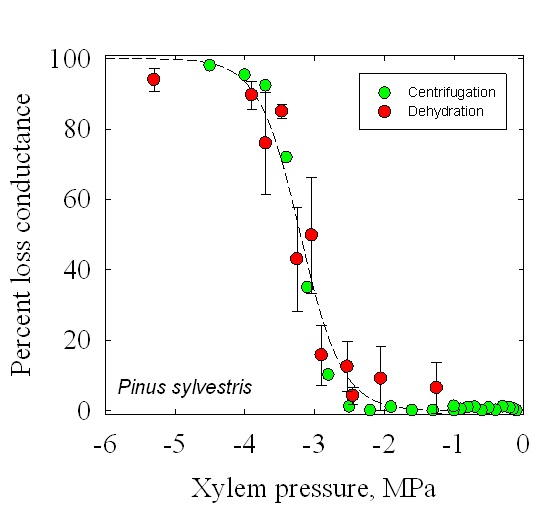
\includegraphics[width = 0.6\tw]{pictures/VC.jpg}\\
\textbf{ Relación de \Blue{potencial hídrico} y \Blue{PLC} de cada nivel de secado}
	\centering{\quelle{\textbf{Ilustración:}   http://prometheuswiki.org}}
\end{frame}

%%%%%%%%%%%%%%%%%%%%%%%%%%%%%%%%%%%%%%%%%%%%%%%%%%%%%%%%%%%%%%%%%%%%%%%%
\section{Referencias}
%%%%%%%%%%%%%%%%%%%%%%%%%%%%%%%%%%%%%%%%%%%%%%%%%%%%%%%%%%%%%%%%%%%%%%%%
\begin{frame}%[allowframebreaks]
\frametitle{Referencias}\label{bib}

\Blue{Basado en un protocolo del Prometheus Wiki que aparentemente ya no está disponible}:

\begin{itemize}
   \item \textbf{Choat, B., Creek, Dk, Lo Gullo M. A., Nardini, A., Oddo, E.,  Raimondo, F., Torres-Ruiz, J. M., Trifilo, P. \& Vilagrosa, A. (2015).} \textit{Prometheus-Wiki - Quantification of vulnerability to xylem embolism - Bench dehydration.} 
\end{itemize}

Un mirror del documento se encuentra en  \url{https://www.researchgate.net/publication/282008335_PrometheusWiki_-_Quantification_of_vulnerability_to_xylem_embolism_-_Bench_dehydration} [revisado 2017-11-26]
\end{frame}
\end{document}
